%%%%%%%%%%%%%%%%%%%%%%%%%%%%%%%%%%%%%%%%%%%%%%%%%%%%%%%
%% Bachelor's & Master's Thesis Template             %%
%% Copyleft by Artur M. Brodzki & Piotr Woźniak      %%
%% Faculty of Electronics and Information Technology %%
%% Warsaw University of Technology, 2019-2020        %%
%%%%%%%%%%%%%%%%%%%%%%%%%%%%%%%%%%%%%%%%%%%%%%%%%%%%%%%

\documentclass[
    left=2.5cm,         % Sadly, generic margin parameter
    right=2.5cm,        % doesnt't work, as it is
    top=2.5cm,          % superseded by more specific
    bottom=3cm,         % left...bottom parameters.
    bindingoffset=6mm,  % Optional binding offset.
    nohyphenation=false % You may turn off hyphenation, if don't like.
]{eiti/eiti-thesis}

\langpol % Dla języka angielskiego mamy \langeng
\graphicspath{{img/}}             % Katalog z obrazkami.
\addbibresource{bibliografia.bib} % Plik .bib z bibliografią

% --- Zmniejszenie odstępów wokół rysunków i tabel ---
% --- Ujednolicenie odstępów wokół rysunków, tabel i listingów ---
\setlength{\intextsep}{10pt plus 2pt minus 2pt}   % Odstęp dla obiektów w tekście [h]
\setlength{\textfloatsep}{10pt plus 2pt minus 2pt} % Odstęp na górze/dole strony
\setlength{\floatsep}{10pt plus 2pt minus 2pt}    % Odstęp pomiędzy dwoma kodami obok siebie
\setlength{\abovecaptionskip}{8pt}                % Odstęp między obiektem a podpisem
\setlength{\belowcaptionskip}{0pt}           % Odstęp pod podpisem            % Odstęp pod podpisem
\raggedbottom
\begin{document}

%--------------------------------------
% Strona tytułowa
%--------------------------------------
\EngineerThesis% Dla pracy inżynierskiej mamy \EngineerThesis
\instytut{Telekomunikacji i Cyberbezpieczeństwa}
\kierunek{Inżynieria Internetu Rzeczy}
%\specjalnosc{Systemy wbudowane i Internet Rzeczy}
\title{
    Rozpoznawanie trików deskorolkowych w aplikacji mobilnej z funkcją mapowania skateparków
}
\engtitle{ % Tytuł po angielsku do angielskiego streszczenia
    Recognition of skateboard tricks in mobile app with skatepark mapping function
}
\author{Jan Błoniarz}
\album{321007}
\promotor{dr inż. Tomasz Mrozek}
\date{\the\year}
\maketitle

%--------------------------------------
% Streszczenie po polsku
%--------------------------------------
\cleardoublepage % Zaczynamy od nieparzystej strony
\streszczenie W niniejszej pracy przedstawiono aplikację mobilną integrującą mapę obiektów sportowych z modułem analizy trików deskorolkowych. System zaprojektowano z uwzględnieniem przetwarzania danych bezpośrednio na urządzeniu końcowym. Do ekstrakcji cech szkieletowych wykorzystano model \textit{Google MoveNet Thunder}, który lokalizuje 17 punktów kluczowych sylwetki. Klasyfikacja sekwencji ruchów opiera się na jednowymiarowej splotowej sieci neuronowej (\textit{1D-CNN}) przekonwertowanej do formatu \textit{TensorFlow Lite}. Warstwę mobilną zaimplementowano w technologii \textit{Flutter}, natomiast warstwę danych i map oparto na usługach \textit{PostgreSQL} oraz \textit{Supabase}. W pracy opisano architekturę systemu, proces przygotowania danych, a także wyniki testów wydajnościowych i funkcjonalnych przeprowadzonych na rzeczywistych urządzeniach.
\slowakluczowe deskorolka, uczenie maszynowe, aplikacja mobilna, wizja komputerowa, praca inżynierska

\newpage
\abstract This thesis presents a mobile application integrating a skatepark map with a skateboarding trick analysis module. The system is designed to perform data processing directly on the edge device. For skeletal feature extraction, the \textit{Google MoveNet Thunder} model is utilized to locate 17 key points of the user's pose. The classification of movement sequences relies on a one-dimensional convolutional neural network (\textit{1D-CNN}) converted into the \textit{TensorFlow Lite} format. The mobile frontend is implemented in \textit{Flutter}, while the database and mapping layer use \textit{PostgreSQL} and \textit{Supabase} services. The thesis describes the system architecture, data preparation process, and the results of performance and functional tests conducted on physical devices.
\keywords skateboard, machine learning, mobile application, computer vision, engineering thesis


%--------------------------------------
% Spis treści
%--------------------------------------
\cleardoublepage % Zaczynamy od nieparzystej strony
\tableofcontents
\newpage
\addtocontents{toc}{\protect\setcounter{tocdepth}{-1}}
\acronymlist
\addtocontents{toc}{\protect\setcounter{tocdepth}{3}}
\acronym{EiTI}{Wydział Elektroniki i Technik Informacyjnych}
\acronym{PW}{Politechnika Warszawska}
\acronym{UI/UX}{ang. \emph{User Interface/User Experience}}
\acronym{SI}{Sztuczna Inteligencja}
\acronym{AI}{ang. \emph{Artificial Intelligence}}
\acronym{IoT}{ang. \emph{Internet of Things}}
\acronym{IMU}{ang. \emph{Inertial Measurement Unit}}
\acronym{HAR}{ang. \emph{Human Action Recognition}}
\acronym{CNN}{ang. \emph{Convolutional Neural Network}}
\acronym{RNN}{ang. \emph{Recurrent Neural Network}}
\acronym{LSTM}{ang. \emph{Long Short-Term Memory}}
\acronym{BLE}{ang. \emph{Bluetooth Low Energy}}
\acronym{API}{ang. \emph{Application Programming Interface}}
\acronym{REST}{ang. \emph{Representational State Transfer}}
\acronym{FPS}{ang. \emph{Frames per second}}
\acronym{API}{ang. \emph{Application Programming Interface}}
%--------------------------------------
% Rozdziały
%--------------------------------------
\cleardoublepage % Zaczynamy od nieparzystej strony
\pagestyle{headings}

\newpage
\section{Wstęp}
        
        W sporcie nie brakuje rozwiązań wspierających uprawianie go - aplikacje, akcesoria, społeczności, fora - biegacze, rowerzyści czy pływacy mogą korzystać z wielu narzędzi do śledzenia i wspierania swojego rozwoju. Nie jest to jednak prawdziwe dla sportów ekstremalnych i \enquote{freestyle'owych}. Na rynku brakuje narzędzi wspierających tych sportowców, pomimo ich rosnącej popularności. Na Igrzyskach Olimpijskich w Tokio w 2020 roku zadebiutowała deskorolka, zyskując tym samym status pełnoprawnego sportu olimpijskiego. Wiąże się to z profesjonalizacją treningów i rosnącym zapotrzebowaniem na narzędzia wspomagające analizę techniczną trików. Dodatkowo, postęp w dziedzinie widzenia komputerowego (ang. \textit{Computer Vision}) daje dziś nowe możliwości tworzenia osobistych, \enquote{kieszonkowych} trenerów, które jeszcze kilka lat temu, wymagałyby zaawansowanego sprzętu z laboratorium biomechaniki.

        Głównym celem pracy inżynierskiej jest stworzenie platformy mobilnej dla społeczności deskorolkowej, która analizuje nagrania trików deskorolkowych, automatycznie je klasyfikuje oraz ocenia poprawność ich wykonania. Ponadto w aplikacji zaimplementowano interaktywną mapę, którą użytkownicy mogą współtworzyć poprzez dodawanie zdjęć oraz informacji o przeszkodach i stanie obiektów. Zaprojektowane rozwiązanie ma na celu wspieranie rozwoju społeczności, umożliwiając jej członkom śledzenie postępów oraz łatwe lokalizowanie nowych miejsc do jazdy.

        W ramach pracy inżynierskiej zrealizowano aplikację mobilną z wykorzystaniem frameworka Flutter (język Dart). W celu realizacji projektu podjęto następujące kroki:
        \begin{enumerate}
            \item Przegląd literatury i rozwiązań istniejących na rynku;
            \item Zdefiniowanie założeń oraz architektury systemu, a także dobór technologii;
            \item Zaprojektowanie interfejsu użytkownika (ang. \textit{User Interface} / \textit{User Experience} [UI/UX]);
            \item Zebranie i przygotowanie zbioru danych wideo;
            \item Wytrenowanie modelu klasyfikacyjnego;
            \item Zaimplementowanie modułu mapy;
            \item Przeprowadzenie testów funkcjonalnych.
        \end{enumerate}
        
        Aplikacja powstała w technologii cross-platformowej, a moduł sztucznej inteligencji działa bezpośrednio na urządzeniu mobilnym (ang. \textit{Edge AI}). Taka decyzja projektowa wynika z fizycznego położenia deskorolkowych \enquote{spotów} -- często znajdują się one w miejscach zurbanizowanych lub ustronnych, do których nie zawsze dociera stabilny zasięg sieci komórkowej. Dzięki uruchamianiu klasyfikatora lokalnie na telefonie, sportowcy mogą korzystać z pełnej analityki wideo w trakcie jazdy, bez konieczności połączenia z Internetem.
        
        W projekcie świadomie zrezygnowano z implementacji mechanizmów uwierzytelniania, ponieważ specyfika rozwiązania nie wymaga tworzenia profili opartych na architekturze chmurowej. Zamiast tego dane przechowywane są lokalnie na urządzeniu, a udostępniana mapa działa w trybie globalnym. Takie podejście pozwoliło uniknąć nadmiarowej złożoności systemu oraz obniżyło próg wejścia, zapobiegając zniechęceniu potencjalnych użytkowników koniecznością zakładania konta przed pierwszym użyciem aplikacji. 

        Z analogicznych względów odstąpiono od integracji zewnętrznych czujników sprzętowych (IoT) montowanych bezpośrednio do deskorolki. Jak wykazała przeprowadzona analiza literatury, rozwiązania oparte wyłącznie na wizji komputerowej są znacznie przystępniejsze, a użytkownicy preferują metody bezinwazyjne. Głównym priorytetem stała się maksymalna ergonomia i prostota obsługi, dzięki czemu smartfon pełni rolę jedynego, w pełni samowystarczalnego narzędzia analitycznego.

        Osobistą motywacją do podjęcia tematu jest zaangażowanie autora pracy w jazdę na deskorolce oraz chęć wsparcia społeczności związanej z tą dyscypliną. Wśród dostępnych narzędzi brakuje rozwiązań wspierających osoby początkujące, dla których obszerne i skomplikowane nazewnictwo trików często stanowi barierę. Ponadto sport ten powszechnie uprawiany jest na ulicznych przeszkodach (tzw. \enquote{spotach}), które nie są oficjalnie skatalogowane jako obiekty sportowe. Brak dostępu do informacji o takich miejscach znacząco utrudnia rozwój umiejętności nowym adeptom tego sportu, ograniczając ich wyłącznie do oficjalnych skateparków. Projekt aplikacji wynika bezpośrednio z osobistych doświadczeń autora i trudności napotkanych na początkowym etapie nauki jazdy na deskorolce.

        Praca inżynierska została podzielona na siedem głównych rozdziałów. Rozdział pierwszy zawiera wstęp, w którym zdefiniowano problem badawczy, motywację autora, cel oraz zakres pracy. Rozdział drugi zawiera przegląd istniejących na rynku aplikacji sportowych dla społeczności deskorolkowej oraz uzasadnia wybór analizy wizyjnej zamiast czujników sprzętowych. W rozdziale trzecim omówiono założenia projektowe, wybór technologii oraz architekturę systemu. Rozdział czwarty jest poświęcony procesowi projektowania interfejsu użytkownika (UI/UX) aplikacji mobilnej. W rozdziale piątym autor skupił się na szczegółowym opisie opracowania modułu sztucznej inteligencji, w tym przygotowanie zbioru danych oraz wybór i trenowanie sieci neuronowej. Rozdział szósty skupia się na technicznych aspektach implementacji aplikacji w środowisku Flutter, tworzeniu modułu mapy oraz integracji z modelem SI. Pracę zamyka rozdział siódmy, zawierający opis przeprowadzonych testów, ewaluację skuteczności modelu rozpoznającego triki oraz końcowe wnioski.
                 % Wygodnie jest trzymać każdy rozdział w osobnym pliku.
\newpage
\section{Przegląd istniejących rozwiązań}

    Poniższy rozdział poświęcono analizie literaturowej oraz przeglądowi rozwiązań dostępnych na rynku. Jego głównym celem jest uzasadnienie kluczowych decyzji projektowych podjętych w pracy, a także zdefiniowanie luki badawczej i rynkowej. W pierwszej kolejności omówiono istniejące aplikacje mobilne dedykowane społeczności deskorolkowej. Następnie przeprowadzono zestawienie metod analizy ruchu w sporcie, porównując zastosowanie czujników sprzętowych z rozwiązaniami opartymi na analizie wideo. W dalszej części przybliżono wybrane modele wizyjnej analizy ruchu. Rozdział zamyka podsumowanie zidentyfikowanych braków w dotychczasowych rozwiązaniach, co stanowi bezpośredni punkt wyjścia dla zaprojektowanego systemu.

    \subsection{Aplikacje dedykowane dla społeczności deskorolkowej}
        Na rynku istnieje kilka rozwiązań dedykowanych społeczności deskorolkowej, które oferują różnorodne funkcje wspierające zarówno początkujących, jak i zaawansowanych użytkowników.

        \medskip
        \noindent\textbf{SkateSpots}
        \medskip
        
            \textit{SkateSpots} to aplikacja umożliwiająca użytkownikom wyszukiwanie i udostępnianie miejsc do jazdy na deskorolce \cite{wikipedia_skatespots}. Użytkownicy mogą dodawać zdjęcia, opisy oraz informacje o przeszkodach i stanie nawierzchni. Narzędzie to posiada również funkcje społecznościowe, takie jak komentowanie i ocenianie poszczególnych lokalizacji. Oprogramowanie nie dysponuje jednak funkcją rozpoznawania trików deskorolkowych i nie zyskało dużej popularności w Polsce.

        \medskip
        \noindent\textbf{FindSkateSpots.com}
        \medskip
        
            Znajdująca się pod adresem \textit{findskatespots.com} platforma internetowa stanowi funkcjonalny odpowiednik aplikacji SkateSpots, przeniesiony do środowiska przeglądarkowego \cite{findskatespots}. Serwis charakteryzuje się stosunkowo niewielką bazą aktywnych użytkowników, skoncentrowaną przede wszystkim w Stanach Zjednoczonych. Z punktu widzenia użyteczności, dedykowana aplikacja mobilna stanowi znacznie wygodniejsze i bardziej przystępne źródło informacji dla przeciętnego deskorolkarza.

        \medskip
        \noindent\textbf{Skatespot.com}
        \medskip
        
            Kolejna platforma internetowa - \textit{skatespot.com} - przeznaczona do lokalizowania skateparków oraz śledzenia aktywności fizycznej \cite{skatespot_home}. Podobnie jak wyżej wymienione rozwiązanie, serwis ten nie został szeroko spopularyzowany wśród docelowej społeczności deskorolkowej.

        \medskip
        \noindent\textbf{Skategrounds}\nopagebreak
        \medskip

            Przykładem rozwiązania komercyjnego o zbliżonych założeniach - czyli dążeniu do automatyzacji procesu dokumentowania postępów treningowych przy jednoczesnym mapowaniu infrastruktury sportowej -  jest platforma \textit{Skategrounds} \cite{skategrounds_tech}. System ten opiera się na architekturze hybrydowej, wykorzystującej dedykowany moduł sprzętowy typu IMU (z ang. \textit{Inertial Measurement Unit}) montowany bezpośrednio do podstawy deskorolki. Czujnik ten komunikuje się bezprzewodowo z aplikacją mobilną, przesyłając dane o przyspieszeniu i orientacji przestrzennej deski w czasie rzeczywistym. Urządzenie, oraz miejsce jego umiejscowienia widoczne jest na rysunku \ref{fig:skategrounds-sensor}.

            \begin{figure}[!h]
                \centering 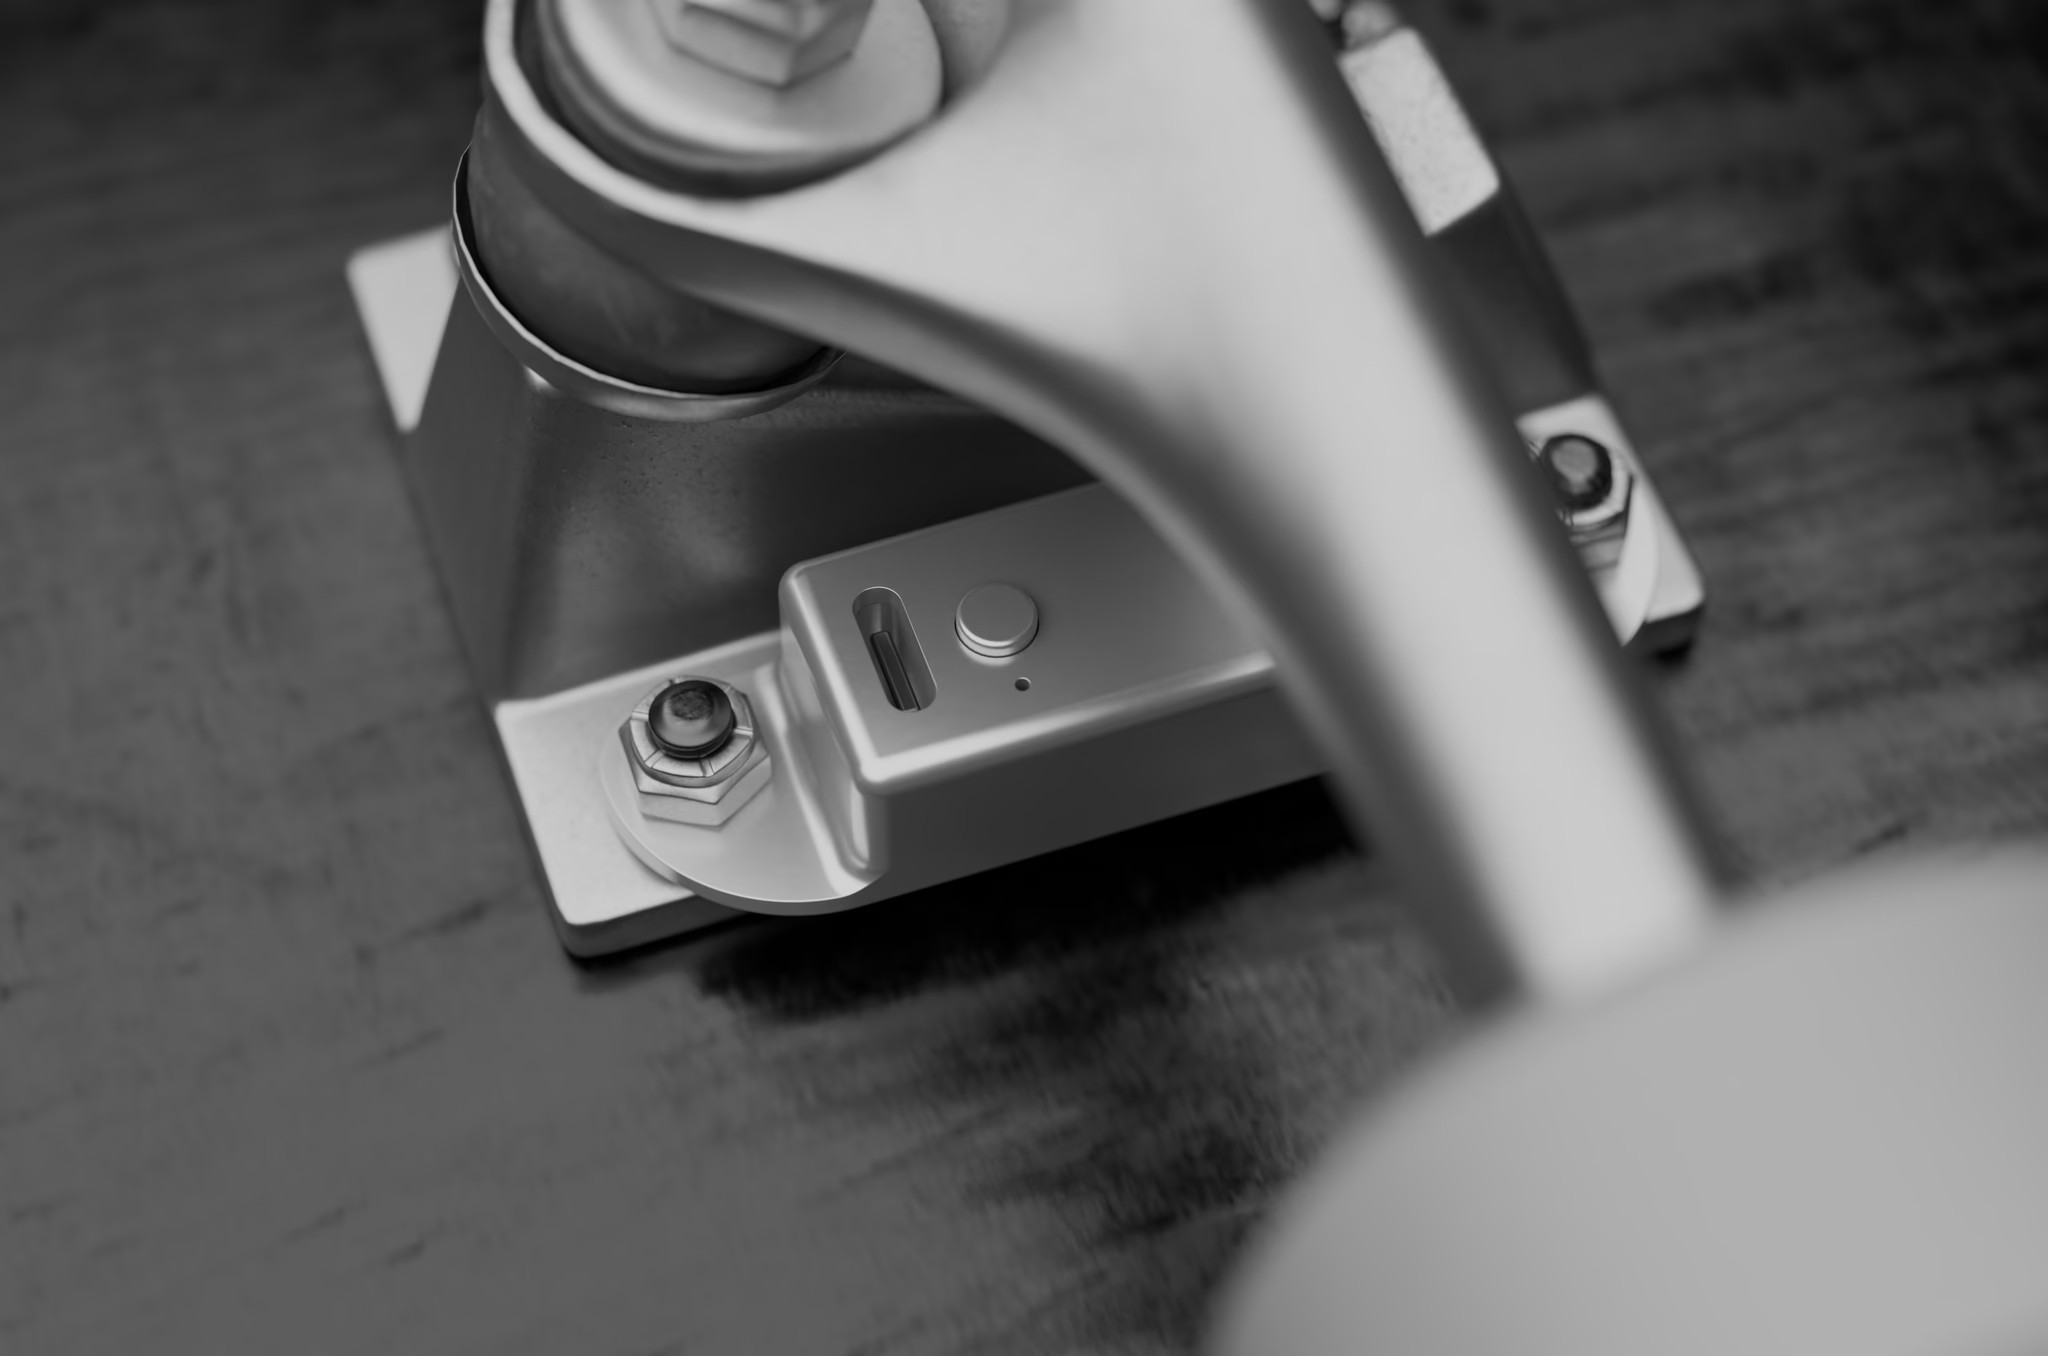
\includegraphics[width=0.5\linewidth]{skategrounds-sensor.jpg}
                \caption{Czujnik \textit{Skategrounds} montowany do podstawy \textit{trucka} deskorolki, Źródło: \cite{skategrounds_tech}.}
                \label{fig:skategrounds-sensor}
            \end{figure}

            Mimo innowacyjnego podejścia, system ten wykazuje istotne ograniczenia natury technicznej. Największą wadą tego podejścia jest brak analizy kinematyki ciała użytkownika. Czujnik rejestryje wyłącznie wektory ruchu samej deskorolki, co powoduje, że algorytmy klasyfikujące nie są w stanie odróżnić rotacji samej deskorolki od rotacji deskorolki wraz z tułowiem skatera. Prowadzi to do niskiej precyzji w rozróżnianiu ewolucji o podobnej charakterystyce ruchu sprzętu, ale różnym ułożeniu ciała (np. Frontside 180$^\circ$, który polega na rotacji zarówno deskorolki, jak i sportowca o 180$^\circ$ przodem do kierunku jazdy, zostanie sklasyfikowany identycznie jak Frontside Shuvit, który polega na rotacji samej deskorolki w tę samą stronę). Ponadto, funkcja mapowania przeszkód sportowych w tej aplikacji ograniczona jest terytorialnie do obszaru Stanów Zjednoczonych, co czyni ją nieużyteczną dla społeczności w innych regionach.

            Eksploatacja zewnętrznego modułu wiąże się również z istotnymi niedogodnościami użytkowymi, takimi jak konieczność regularnego ładowania ogniwa zasilającego. Ponadto, użytkownik jest zmuszony do stałego dbania o stan techniczny sensora. Ze względu na inwazyjne miejsce montażu — bezpośrednio na konstrukcji deskorolki — urządzenie jest narażone na trudne warunki zewnętrzne. Brak pełnej odporności na wilgoć sprawia, że przypadkowy kontakt z wodą (np. przejazd przez kałużę) może doprowadzić do permanentnego uszkodzenia elektroniki, co w konsekwencji uniemożliwia dalsze korzystanie z systemu. Powyższe czynniki stanowią dodatkową barierę, która często zniechęca sportowców do wyboru rozwiązań opartych na czujnikach sprzętowych.

        \medskip
        \noindent\textbf{Spinnax}
        \medskip

            Kolejnym rozwiązaniem komercyjnym o charakterystyce zbliżonej do platformy \textit{Skategrounds} jest system \textit{Spinnax FREAK}, opracowany przez niemiecki start-up \cite{spinnax_com}. Urządzenie wykorzystuje moduł sprzętowy montowany pod podstawą \textit{trucka} deskorolki, który w odróżnieniu od swojego poprzednika charakteryzuje się pełną wodoodpornością, co minimalizuje ryzyko awarii wynikających z kontaktu z wilgocią. Zasada działania opiera się na integracji dedykowanego sensora o gabarytach przekraczających wymiary modułu \textit{Skategrounds} z aplikacją mobilną za pośrednictwem protokołu bezprzewodowego. System umożliwia rejestrację historii przejazdów w czasie rzeczywistym oraz udostępnia moduł automatycznego nazewnictwa i analizy wykonanych ewolucji. Dodatkową funkcjonalnością jest tryb odtwarzania sekwencji ruchu \enquote{krok po kroku}, pozwalający użytkownikowi na manualną weryfikację techniki wykonania triku. Zdjęcie urządzenia wraz ze zrzutem ekranu z aplikacji mobilnej widoczne jest na rysunku \ref{fig:spinnax}.

            \begin{figure}[!h]
                \centering 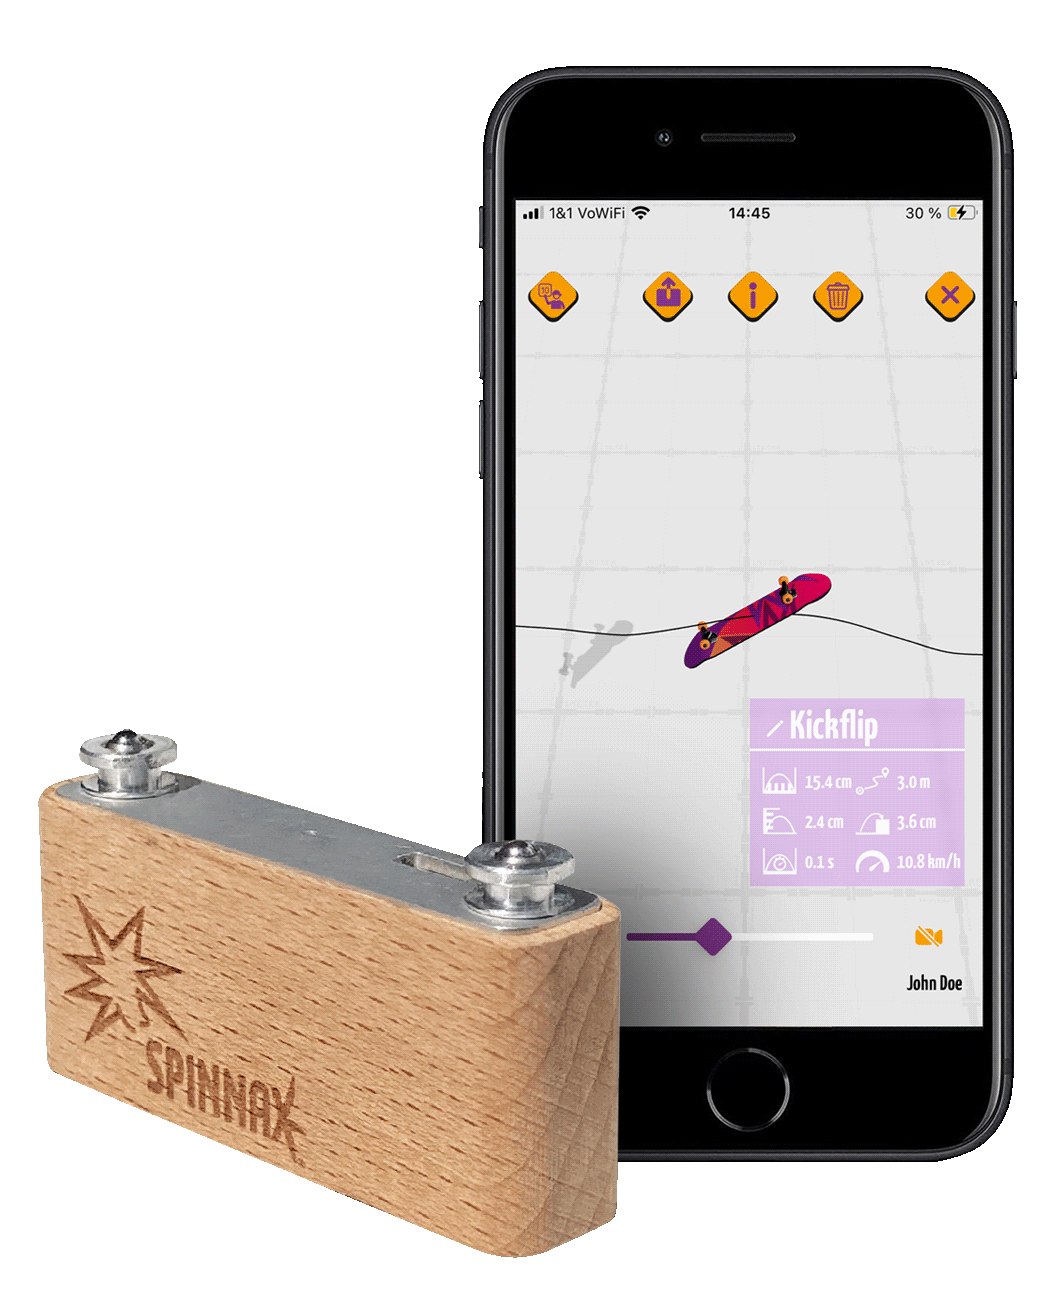
\includegraphics[width=0.5\linewidth]{spinnax.png}
                \caption{Urządzenie \textit{Spinnax FREAK} oraz dedykowana aplikacja mobilna, Źródło: \cite{spinnax_com}.}
                \label{fig:spinnax}
            \end{figure}           
            
            Mimo usprawnień w zakresie ochrony fizycznej urządzenia, platforma wykazuje istotne ograniczenia natury technicznej i rynkowej. Podobnie jak w przypadku innych systemów opartych wyłącznie na czujnikach kinematycznych, rozwiązanie to wykazuje niską precyzję w klasyfikacji ewolucji opartych na rotacji ciała użytkownika, co wynika z braku wizyjnej analizy sylwetki skatera. Użyteczność systemu jest dodatkowo ograniczona barierą językową - interfejs aplikacji dostępny jest wyłącznie w języku niemieckim, co znacząco zawęża potencjalne grono odbiorców. Ponadto platforma nie oferuje funkcji mapowania infrastruktury sportowej, co ogranicza jej rolę w budowaniu społeczności. Krytycznym aspektem z punktu widzenia użytkownika końcowego jest model biznesowy oparty na cyklicznej subskrypcji lub wysokiej opłacie początkowej. Wysoki koszt eksploatacji w stosunku do oferowanych możliwości analitycznych stanowi istotną barierę adopcji tego rozwiązania na rynku masowym.

    \subsection{Analiza ruchu w sporcie: Wideo a czujniki sprzętowe}
        Rozpoznawanie ludzkich akcji (z ang. \textit{Human Action Recognition - HAR}) w sporcie polega na wykrywaniu atlety, śledzeniu jego ruchów oraz identyfikacji rodzaju wykonywanej czynności \cite{host2022overview}. Jak wskazują Host i Ivašić-Kos \cite{host2022overview} w swoim przeglądzie, głównym celem systemów HAR jest nie tylko prosta klasyfikacja ruchu, ale również automatyzacja analizy statystycznej oraz monitorowanie wydajności sportowców w celu poprawy ich techniki\cite{host2022overview}.

        Wybór analizy wizyjnej zamiast systemów opartych na czujnikach sprzętowych (takich jak moduły IMU) jest uzasadniony kilkoma czynnikami technologicznymi:
        \begin{itemize}
            \item \textbf{Bezinwazyjność i dostępność}: Ze względu na wykorzystanie danych wizualnych, stosowanie systemów opartych na wizji komputerowej eliminuje konieczność montowania sensorów na każdym stawie zawodnika, co może być konieczne w przypadku precyzyjnych systemów inercyjnych \cite{host2022overview}.
            \item \textbf{Kompleksowość danych}: Nowoczesne biblioteki, takie jak \textit{TensorFlow} czy \textit{OpenCV} dostarczają szeroką gamę gotowych algorytmów uczenia maszynowego. Pozwala to na automatyczną ekstrakcję cech zamiast ręcznego projektowania deskryptorów, co było domeną starszych metod \cite{host2022overview}.
        \end{itemize}

        Mimo tych zalet, implementacja HAR w sporcie wiąże się z wyzwaniami takimi jak okluzja, dynamiczne tło oraz konieczność śledzenia wielu osób jednocześnie, co wymaga zastosowania zaawansowanych modeli klasy uczenia maszynowego \cite{host2022overview}.

        Historycznie śledzenie ruchu zawodników opierało się na analizie notacyjnej (ang. \textit{notational analysis}), polegającej na subiektywnej ocenie obserwatora. Był to proces ograniczony do niewielkiej liczby badanych osób i czasochłonny. Współczesna metrologia sportowa dąży do uzyskiwania obiektywnych, ilościowych profili prędkości oraz przyspieszenia co pozwala na głębsze zrozumienie dynamiki koordynacji i strategii taktycznych \cite{barris2008review}.

        Pomimo wysokiej precyzji pomiarowej czujników inercyjnych i akcelerometrów, ich praktyczne zastosowanie w warunkach sportowych napotyka na istotne bariery:
        \begin{itemize}
            \item \textbf{Bezpieczeństwo i regulacja}: Barris i Button \cite{barris2008review} zauważają, że czujniki noszone przez sportowców są często niedopuszczane do użytku podczas oficjalnych zawodów i meczów ze względu na restrykcyjne przepisy oraz potencjalne ryzyko kontuzji zawodnika \cite{barris2008review}.
            \item \textbf{Logistyka i motoryka}: Jak wskazują Ahmadi i inni \cite{ahmadi2015toward}, dla rzetelnej oceny ruchu konieczne jest precyzyjne umieszczanie sensorów na każdym stawie będącym przedmiotem zainteresowania. Proces ten nie tylko jest uciążliwy, ale ingeruje również w naturalne wzorce ruchowe sportowca, co jest szczególne istotne w dyscyplinach wymagających wysokiej zwinności. W przypadku deskorolki, czujniki umieszczane bezpośrednio na niej wpływają na jej wymiary oraz ciężar, co również może mieć wpływ na osiągi atlety \cite{ahmadi2015toward}.
            \item \textbf{Koszty sprzętowe}: W przeciwieństwie do systemów wizyjnych, które mogą wykorzystywać instniejącą infrastrukturę wideo (np. smartfon), systemy oparte na czujnikach wymagają znacznych nakładów na specjalistyczny sprzęt oraz dedykowane zaplecze obliczeniowe \cite{barris2008review}.
        \end{itemize}

        Decyzja o wykorzystaniu metod wizyjnych w procesie HAR jest podyktowana potrzebą uzyskania obiektywnych danych, przy jednoczesnym zachowaniu pełnej swobody ruchu sportowca. Ingerowanie w środowisko treningowe zawodników, może mieć negatywny wpływ na ich osiągi. Mimo, że zarówno analiza wizyjna, jak i czujnikowa dążą do tego samego celu, różnią się one znacząco pod względem logistyki wdrożenia oraz wpływu na bezpieczeństwo atlety. Zbiorcze zestawienie kluczowych różnic funkcjonalnych i technicznych pomiędzy tymi metodami przedstawiono w tabeli \ref{tab:porownanie_metod}.

        \begin{table}[!h]
            \centering
            \caption{Porównanie wizyjnej i czujnikowej analizy ruchu w sporcie, Źródło [opracowanie własne].}
            \label{tab:porownanie_metod}
            \small
            % tabela lepiej zeby byla na tej samej stronie, zle to wyglada
            \begin{tabularx}{\textwidth} {| >{\raggedright\arraybackslash}p{4.2cm} | >{\RaggedRight\arraybackslash}X | >{\RaggedRight\arraybackslash}X |} \hline
                \textbf{Kryterium} & \textbf{Analiza wizyjna (Wideo)} & \textbf{Analiza czujnikowa (IMU)} \\ \hline
                \textbf{Inwazyjność} & Bezinwazyjna (marker-less), wykorzystuje istniejące dane wizualne \cite{barris2008review, host2022overview}. & Wymaga fizycznego montażu sensorów na ciele lub sprzęcie \cite{barris2008review}. \\ \hline
                \textbf{Wpływ na motorykę} & Brak ingerencji w naturalne wzorce ruchowe sportowca \cite{ahmadi2015toward}. & Możliwe zakłócenie ruchu przez czujniki lub okablowanie \cite{ahmadi2015toward}. \\ \hline
                \textbf{Bezpieczeństwo} & Całkowicie bezpieczna dla atlety \cite{barris2008review}. & Ryzyko kontuzji; czujniki często niedopuszczane do oficjalnych zawodów \cite{barris2008review}. \\ \hline
                \textbf{Logistyka} & Wysoka (np. smartfon); brak konieczności żmudnej kalibracji stawów \cite{host2022overview}. & Uciążliwa; wymaga precyzyjnego umieszczenia sensorów na każdym stawie \cite{ahmadi2015toward}. \\ \hline
                \textbf{Koszty} & Niskie; wykorzystanie powszechnej infrastruktury wideo \cite{barris2008review}. & Wysokie nakłady na specjalistyczny sprzęt i zaplecze obliczeniowe \cite{barris2008review}. \\ \hline
                \textbf{Główne wyzwania} & Okluzja, dynamiczne tło, zmiany oświetlenia \cite{barris2008review, host2022overview}. & Błędy dryfu, konieczność rekalibracji, bariery regulaminowe \cite{barris2008review, ahmadi2015toward}. \\ \hline
            \end{tabularx}
        \end{table}

        Przejście na zautomatyzowaną analizę wizyjną stwarza jednak własne wyzwania techniczne. Specyfika ruchu w sporcie, charakteryzująca się gwałtownymi zmianami kierunku, wysoką dynamiką oraz, w przypadku sportów zespołowych, kolizjami między zawodnikami, narusza podstawowe założenia o \enquote{płynności ruchu}, na których opierają się klasyczne algorytmy śledzące. Według Barris i Button, głównym wyzwaniem pozostaje stabilna identyfikacja i etykietowanie osób w zatłoczonym środowisku, gdzie jakość obrazu, zmiany oświetlenia oraz okluzja utrudniają nieprzerwany monitoring ewolucji \cite{barris2008review}. Pomimo, że deskorolka nie jest sportem zespołowym, w środowisku zawodów bądź na skateparku, wcześniej wspomniane problemy jak najbardziej występują. Z tych powodów współcześnie badania koncentrują się na metodach głębokiego uczenia, które dzięki automatyzacji ekstrakcji cech pozwalają na coraz skuteczniejszą interpretację zachowań w dynamicznych scenach sportowych. 

    \subsection{Modele wizyjnej analizy ruchu}
        
        Ewolucja metod wizyjnych w sporcie rozpoczęła się od systemów śledzenia opierających się na detekcji ruchu i statystycznych modelach kształtu. Klasyczne podejścia wykorzystywały tzw. reprezentację typu \enquote{blob}, która polega na grupowaniu pikseli o podobnych właściwościach spektralnych w celu wyodrębnienia sylwetki zawodnika z tła \cite{barris2008review}. Jednym z wczesnych systemów tego typu był \textit{Pfinder}, który interpretował ruch człowieka przy użyciu wieloklasowych modeli statystycznych koloru i kształtu, choć jego skuteczność drastycznie spadała w przypadku wielu zawodników.

        Przełomem w dziedzinie HAR stało się zastosowanie głębokiego uczenia, które pozwoliło na pełną automatyzację ekstrakcji cech. Współczesne architektury można sklasyfikować według ich roli w przetwarzaniu danych wideo \cite{host2022overview}:
        \begin{itemize}
            \item \textbf{Splotowe sieci neuronowe (CNN)}: Wykorzystywane jako klasyfikatory typu \textit{end-to-end}. W analizie sportowej dwuwymiarowe sieci CNN (2D-CNN) służą do ekstrakcji cech przestrzennych z pojedynczych klatek, natomiast trójwymiarowe (3D-CNN) przechwytują informacje czasowo-przestrzenne, co jest kluczowe dla zrozumienia dynamiki ruchu \cite{host2022overview}.
            \item \textbf{Sieci rekurencyjne (RNN) i LSTM}: Te architektury są projektowane z myślą o przetwarzaniu sekwencji danych, co czyni je idealnymi do analizy wideo klatka po klatce. Sieci LSTM (ang. \textit{Long Short-Term Memory}) wykorzystują specjalne jednostki pamięci do przechowywania stanów czasowych. Pozwala to na klasyfikację złożonych ruchów trwających od kilku do kilkunastu sekund \cite{host2022overview}.
            \item \textbf{Transformery i mechanizmy uwagi}: Najnowszy trend w badaniach nad HAR, pozwalający na lepsze wychwytywanie długoterminowych zależności niż tradycyjne sieci RNN. Zawdzięcza to mechanizmowi samo-uwagi, który uczy się skupiać na najistotniejszych regionach obrazu (np. kończynach zawodnika) w kontekście całej sceny \cite{host2022overview}.
        \end{itemize}

        W analizie dyscyplin technicznych i ekstremalnych, takich jak deskorolka, kluczowe znaczenie ma estymacja pozy. Polega ona na ekstrakcji kluczowych punktów szkieletu, najczęściej stawów. Istnieją na rynku rozwiązania, takie jak \textit{OpenPose}, które pozwalają na uzyskanie precyzyjnych danych o ruchach sportowca bez konieczności stosowania znaczników na jego ciele \cite{openpose2025}. Wybór konkretnego modelu (np. z rodziny \textit{MobileNet} lub \textit{ResNet}) jest zawsze podyktowany kompromisem między dokładnością, a wydajnością obliczeniową, co jest szczególnie istotne w przypadku aplikacji mobilnych działających w czasie rzeczywistym \cite{host2022overview}. 

        Przykładem nowoczesnego rozwiązania, które bezpośrednio implementuje zasady optymalizacji opisane przez Host i Ivašić-Kos, jest model \textit{Google MoveNet} \cite{movenet2021}. Wykorzystuje on bibliotekę \textit{TensorFlow}, o której autorki wspominają jako o jednym z kluczowych narzędzi umożliwiających szybki rozwój projektów wizyjnych bez konieczności ich budowy od podstaw \cite{host2022overview}. \textit{MoveNet}, opierając się na architekturze CNN, został zaprojektowany z myślą o urządzeniach o ograniczonej mocy obliczeniowej, biorąc pod uwagę rygorystyczny kompromis między dokładnością i szybkością działania. Takie założenia projektowe powodują, że model ten jest zoptymalizowany pod uruchomienie na urządzeniach mobilnych. Dzięki bezmarkerowej ekstrakcji punktów kluczowych, model ten radzi sobie z wyzwaniami okluzji, dynamicznego i nieustrukturyzowanego tła, wspominanych przez Barris i Button jako jedne z głównych barier tradycyjnych systemów śledzących \cite{barris2008review}. Dodatkowo, \textit{MoveNet} oferuje dwa warianty swojego modelu: \textit{Thunder}, który priorytetyzuje dokładność oraz \textit{Lightning}, w którym większe znaczenie ma szybkość obliczeń. Taki wybór pozwala dostosować model do konkretnego zastosowania \cite{movenet2021}.
        
    \subsection{Podsumowanie}
        Przeprowadzony przegląd istniejących rozwiązań oraz stanu sztuki, wskazuje na postępujący rozwój metod monitorowania sportu - od analizy notacyjnej, w której obserwatorem był człowiek, po zaawansowane systemy automatycznego śledzenia ruchu. W obszarze dyscyplin ekstremalno-technicznych, takich jak deskorolka, wciąż widoczny jest podział na precyzyjne, lecz inwazyjne i kosztowne systemy sprzętowe oraz ogólnodostępne, ale mało zaawansowane platformy społecznościowe.

        Kluczowe wnioski z powyższego rozdziału można ująć w następujących punktach:
        \begin{itemize}
            \item \textbf{Ograniczenia systemów inercyjnych}: Pomimo wysokiej dokładności, korzystanie z rozwiązań opartych na czujnikach wiąże się z koniecznością montażu dodatkowego sprzętu na deskorolce, co ingeruje w naturalną motorykę sportowca i wyważenie deski. W przypadku rozwiązań takich jak \textit{Skategrounds} użytkownik musi mieć stale na uwadze obecność czujnika, w przeciwnym wypadku może doprowadzić do permanentnego uszkodzenia kosztownego sprzętu.
            \item \textbf{Bariery ekonomiczne i regulacyjne}: Profesjonalne systemy wizyjne i czujnikowe wymagają wysokich nakładów pieniężnych i sprzętowych, co ogranicza ich dostępnosć do wąskiej grupy profesjonalistów. Wiele z tych urządzeń nie może być również wykorzystywanych w profesjonalnym środowisku, takim jak zawody sportowe.
            \item \textbf{Potencjał technologii HAR}: Nowoczesne algorytmy HAR oparte na głębokim uczeniu, takie jak architektury CNN, czy modele estymacji pozy (np. \textit{Google MoveNet}), pozwalają na automatyczną ekstrakcję cech bezpośrednio z obrazu wideo. Eliminuje to potrzebę stosowania markerów i czujników, tym samym znacząco ułatwiając zarówno uprawianie sportu, jak i monitorowanie zawodnika.
        \end{itemize}

        Podsumowując, na rynku brakuje kompleksowego rozwiązania, które integrowałoby funkcję mapowania infrastruktury sportowej z bezinwazyjną zaawansowaną analizą techniczną trików realizowaną w czasie rzeczywistym na urządzeniu mobilnym. Większość istniejących aplikacji skupia się albo na aspekcie lokalizacyjnym, albo na klasyfikacji ruchu opartej o czujniki sprzętowe, podatne na fizyczne uszkodzenia oraz ingerujące w osiągi sportowca. Niniejszy projekt ma na celu wypełnienie tej luki poprzez implementację platformy do analizy wizyjnej oraz mapowania infrastruktury sportowej, zoptymalizowanej pod urządzenia mobilne. Pozwoli to na obiektywną ocenę postępów treningowych bez nakładów finansowych na dodatkowy sprzęt.
            % Umożliwia to również łatwą migrację do nowej wersji szablonu:
\newpage
\section{Założenia i architektura systemu}
    Niniejszy rozdział stanowi szczegółowy opis opracowania architektury aplikacji moblilnej integrującej system mapowania infrastruktury sportowej z modułem SI klasyfikującym triki deskorolkowe. Projektowanie systemu poprzedzono porównaniem różnych podejść technologicznych rozważanych przez autora na etapie planowania pracy.

    \subsection{Wymagania funkcjonalne i niefunkcjonalne}

        Wymagania projektowe stanowią fundament modelowania systemu, pozwalający na obiektywną ocenę realizacji założonych celów inżynierskich oraz optymalny dobór technologii pod kątem scenariuszy użycia. W literaturze przedmiotu wymagania te dzieli się na funkcjonalne, opisujące konkretne operacje systemu, oraz niefunkcjonalne, definiujące jakość i parametry jego działania.

        \textbf{Wymagania funkcjonalne} określają kluczowe operacje, jakie system musi wykonywać w celu wsparcia treningu deskorolkowego:
        \begin{itemize}
            \item Rejestracja oraz odczyt materiałów wideo zawierających ewolucje sportowe;
            \item Automatyczna klasyfikacja trików z wykorzystaniem algorytmów głębokiego uczenia w celu poprawy techniki zawodnika;
            \item Udostępnianie interaktywnej mapy obiektów sportowych („spotów”) wraz z funkcją ich edycji i dodawania nowych lokalizacji;
            \item Prowadzenie lokalnej bazy danych zawierającej historię postępów i wykonanych ewolucji.
        \end{itemize}

        \textbf{Wymagania niefunkcjonalne} definiują ograniczenia techniczne i jakościowe, które są niezbędne do zachowania bezinwazyjnego charakteru analizy:
        \begin{itemize}
            \item Realizacja obliczeń modułu klasyfikacji w paradygmacie Edge AI (lokalnie na urządzeniu), co umożliwia pracę w miejscach o ograniczonym zasięgu sieciowym;
            \item Minimalizacja latencji procesu analizy wizyjnej, zapewniająca niemal natychmiastową informację zwrotną dla sportowca;
            \item Pełna bezinwazyjność – system nie może wymagać posiadania dodatkowych sensorów ani markerów, co gwarantuje zachowanie naturalnej motoryki ruchu;
            \item Przejrzystość interfejsu użytkownika oraz wysoki poziom użyteczności modułu mapy.
        \end{itemize}

        Precyzyjne zdefiniowanie powyższych priorytetów determinuje wybór architektury oraz stosu technologicznego wykorzystanego w dalszej części pracy.
    \subsection{Wybór technologii}

        Proces wyboru technologii opierał się na weryfikacji dwóch skrajnych koncepcji architektury sprzętowo programowej. Wstępne założenia projektowe zakładału wykorzystanie zewnętrzych czujników inercyjnych montowanych bezpośrednio na deskorolce. Na dalszym etapie rozwoju projektu zdecydowano się na podejście analizy wizyjnej, z powodów szerzej rozwiniętych w drugim rozdziale pracy inżynierskiej.

        \subsubsection{Podejście IoT (czujnikowe)}

            W pierwszej fazie rozważano system typu IoT, w którym mikrokontroler (np. ESP32) agregowałby dane z akcelerometru i żyroskopu, przesyłając je do dedykowanego \textit{backendu} opartego na frameworku \textit{FastAPI} za pośrednictwem protokołu \textit{Bluetooth Low Energy} (BLE). Schemat takiego rozwiązania przedstawiono na rysunku \ref{fig:schemat-iot}.

            \begin{figure}[!h]
                \centering 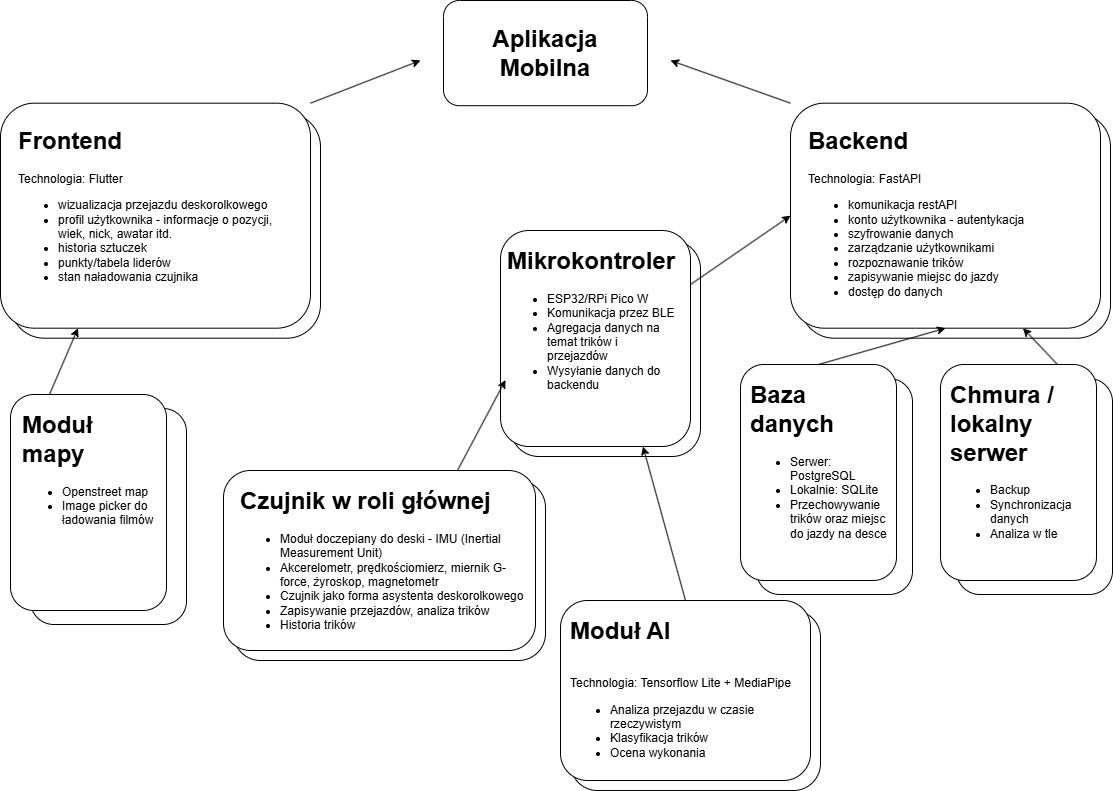
\includegraphics[width=\linewidth]{Schemat2.png}
                \caption{Schemat czujnikowej architektury systemu, Źródło: [Opracowanie własne].}
                \label{fig:schemat-iot}
            \end{figure}

            Koncepcja ta została rozwinięta w stronę rozwiązania hybrydowego, w którym dane czujnikowe miały służyć jako multimodalny zbiór danych wspierający proces trenowania klasyfikatora. W tym scenariuszu użytkownik końcowy korzystałby wyłącznie z analizy wizyjnej, co eliminowałoby potrzebę montażu dodatkowych urządzeń na sprzęcie sportowym. Zmodyfikowany schemat architektury systemu widoczny jest na rysunku \ref{fig:schemat-czujnik}.

            \begin{figure}[!h]
                \centering 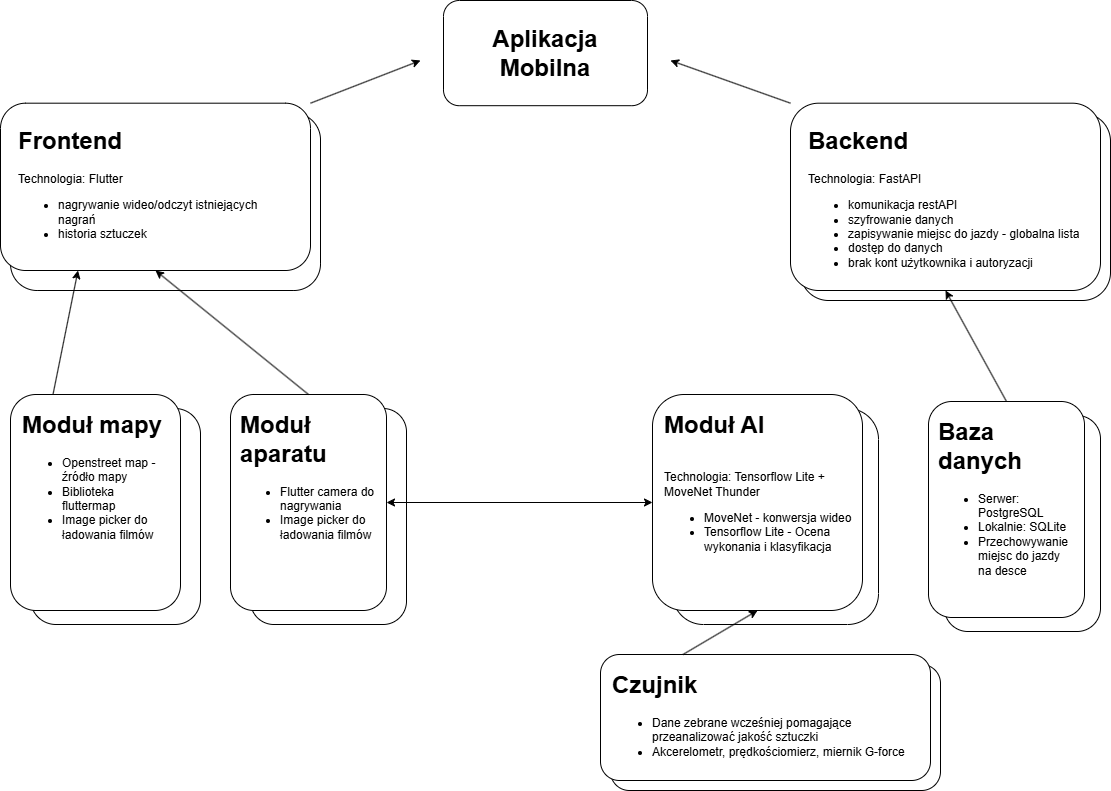
\includegraphics[width=\linewidth]{Schemat5.png}
                \caption{Schemat hybrydowej architektury systemu, Źródło: [Opracowanie własne].}
                \label{fig:schemat-czujnik}
            \end{figure}   
            
            Biorąc jednak pod uwagę bariery logistyczne oraz ryzyko uszkodzenia elektroniki eksploatowanej w trudnych warunkach zewnętrznych, obie koncepcje uznano za nieefektywne. Jak wykazała analiza literatury, sensory montowane bezpośrednio na deskorolce nie pozwalają na analizę ruchu poszczególnych stawów sportowca, co drastycznie obniża precyzję klasyfikacji ewolucji opartych na złożonej rotacji ciała. Wykorzystanie danych czujnikowych jedynie w fazie treningowej również wiązało się z istotnymi wyzwaniami merytorycznymi. Brak obiektywnych wzorców odniesienia wymuszałby oparcie procesu etykietowania danych na analizie notacyjnej, czyli subiektywnej ocenie obserwatora. Taka metodologia jest nie tylko czasochłonna, ale również obarczona błędem ludzkim, co w kontekście budowy rzetelnego systemu automatycznego rozpoznawania akcji (HAR) czyni ją niemiarodajną pod względem naukowym i technicznym. 

        \subsubsection{Podejście wizyjne (\textit{Edge AI})}
                    
            W opozycji do systemów inercyjnych, ostateczna koncepcja systemu została oparta na paradygmacie analizy wizyjnej realizowanej w całości na urządzeniu mobilnym (ang. \textit{on-device processing}). Wybór ten podyktowany był dążeniem do pełnej bezinwazyjności pomiarowej, wskazywanej jako kluczowy warunek zachowania naturalnej motoryki ruchu sportowca. Architektura ta, przedstawiona na rysunku \ref{fig:schemat-har}, stanowi implementację systemu HAR, który eliminuje błędy wynikające z braku analizy ułożenia ciała użytkownika.

            Warstwa prezentacji oraz logika biznesowa aplikacji zostały zaimplementowane w frameworku \textit{Flutter}, co zapewnia wysoką wydajność interfejsu przy zachowaniu wieloplatformowości kodu źródłowego. Moduł mapy, kluczowy dla funkcji lokalizowania obiektów sportowych, oparto na bibliotece \textit{flutter\_map}. Wykorzystuje ona dane z otwartego projektu \textit{OpenStreetMap}, co pozwala na elastyczne zarządzanie warstwami wizualnymi i keszowanie kafelków mapy, zwiększając użyteczność systemu w warunkach ograniczonej łączności sieciowej.

            Najistotniejszym elementem technologicznym jest silnik analityczny wykorzystujący bibliotekę \textit{TensorFlow Lite} – zoptymalizowane środowisko uruchomieniowe dla modeli uczenia maszynowego na systemy wbudowane i mobilne. Za proces ekstrakcji cech przestrzennych odpowiada model \textit{Google MoveNet} w wariancie \textit{Thunder}. Został on wybrany ze względu na rygorystyczny kompromis pomiędzy wysoką precyzją lokalizacji punktów kluczowych (stawów), a ograniczonymi zasobami sprzętowymi smartfonów. Tak skonstruowany potok przetwarzania danych (ang. \textit{data pipeline}) pozwala na bezmarkerowe śledzenie sylwetki w czasie rzeczywistym, co stanowi fundament dla warstwy klasyfikacyjnej trików deskorolkowych.

            \begin{figure}[!h]
                \centering 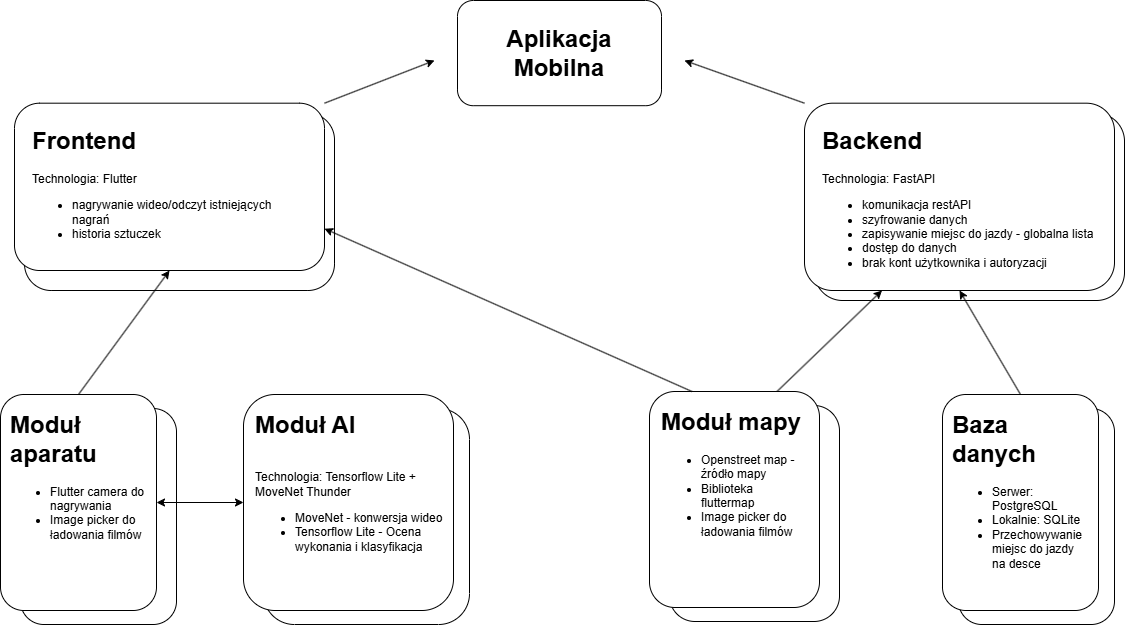
\includegraphics[width=\linewidth]{Schemat3.png}
                \caption{Schemat wizyjnej architektury systemu, Źródło: [Opracowanie własne].}
                \label{fig:schemat-har}
            \end{figure}     

    \subsection{Architektura systemu}

        Docelowa struktura aplikacji, widoczna na rysunku \ref{fig:schemat-har}, opiera się na realizacji możliwie jak największej ilości procesów logicznych bezpośrednio na urządzeniu mobilnym. Takie zdecentralizowane podejście gwarantuje najwyższy poziom prywatności danych oraz niezawodność systemu w miejscach o ograniczonym zasięgu sieci komórkowej. Struktura aplikacji została podzielona na kilka współpracujących ze sobą modułów.

        Głównym elementem interfejsu jest \textit{frontend}, opracowany w technologii \textit{Flutter}, który odpowiada za nagrywanie i odczyt materiałów wideo, prezentację historii wykonanych ewolucji oraz umożliwienie użytkownikowi korzystanie z mapy skateparków i przeszkód. Dane wejściowe dostarczane są przez moduł aparatu, który umożliwia rejestrację obrazu przy użyciu biblioteki \textit{camera} lub wybór istniejących nagrań za pomocą komponentu \textit{image picker}. Nagranie trafia następnie do modułu SI, gdzie model \textit{MoveNet} dokonuje ekstrakcji pozy. Skonwertowany materiał jest klasyfikowany i oceniany z wykorzystaniem \textit{TensorFlow Lite}. Realizacja tych procesów bezpośrednio na urządzeniu pozwala na szybką identyfikację triku bez konieczności przesyłania dużych plików do zewnętrznego serwera.

        Za aspekt społecznościowy i współdzielenie danych odpowiada moduł mapy, integrujący bibliotekę \textit{flutter\_map} z danymi \textit{OpenStreetMap}. Komunikuje się on z backendem zaimplementowanym w języku \textit{Python}, z wykorzystaniem frameworku \textit{FastAPI}. Warstwa serwerowa zarządza globalną listą miejsc do jazdy, zapewnia szyfrowanie danych oraz udostępnia zasoby przez protokół \textit{REST API} (z ang. \textit{Representational State Transfer Application Programming Interface}). Zgodnie z założeniami projektowymi, system zapewnia dostę do danych bez konieczności tworzenia kont użytkowników i autoryzacji, tym samym znacząco obniżając próg wejścia dla społeczności. Warstwę trwałości danych stanowi baza danych, wykorzystująca serwer \textit{PostgreSQL} do zarządzania zasobami globalnymi (listą \enquote{spotów} deskorolkowych) oraz lokalną bazę \textit{SQLite} do przechowywania historii trików bezpośrednio na urządzeniu.
\newpage
\section{Projekt interfejsu użytkownika}
    Niniejszy rozdział opisuje proces projektowania warstwy prezentacji aplikacji mobilnej, ze szczególnym uwzględnieniem zasad użyteczności oraz specyfiki środowiska, w jakim system będzie eksploatowany. Głównym celem projektowym na tym etapie prac było stworzenie intuicyjnego interfejsu, który umożliwi sportowcom intuicyjne znajdowanie miejsc do jazdy oraz szybki dostęp do funkcji analitycznych, bez konieczności przerywania sesji treningowej.

    Istotnym założeniem tego etapu było rozdzielenie fazy koncepcyjnej i prototypowania od samej implementacji kodu źródłowego aplikacji. Umożliwiło to skupienie się na ergonomii i logice \textit{UI/UX} przed przystąpieniem do prac programistycznych, opisanych szczegółowo w rozdziale szóstym.
    
    \subsection{Założenia projektowe i makiety aplikacji}

        Proces projektowania interfejsu oparto na paradygmacie projektowania zorientowanego na użytkownika. Głównym narzędziem wykorzystywanym do stworzenia makiet aplikacji było środowisko \textit{Figma}. Za jego pomocą wypracowano wstępny układ elementów graficznych oraz prototyp interakcji z użytkownikiem przed ich wdrożeniem w środowisku \textit{Flutter}.

        Należy podkreślić, że makiety powstałe na tym etapie pracy inżynierskiej stanowią idealizację systemu. Służyły one przede wszystkim jako punkt odniesienia podczas projektowania rzeczywistego interfejsu. Finalny produkt różni się w pewnym stopniu od prototypów zaprezentowanych w tym rozdziale, co wynika z technicznych ograniczeń bibliotek mobilnych oraz optymalizacji interfejsu pod kątem wydajności na urządzeniach o mniejszej mocy obliczeniowej. W tej części pracy przedstawiono wizję projektową i założenia estetyczne, a rzeczywisty wygląd oraz techniczne detale wdrożonych komponentów zostały przedstawione w rozdziale poświęconym implementacji aplikacji.

        Jako komercyjną nazwę aplikacji wybrano angielskie słowo \textit{Flatground}, pisane wielkimi literami. Oznacza ono w dosłownym tłumaczeniu płaską ziemię, natomiast w slangu deskorolkowym, słowo to figuruje jako określenie płaskiego miejsca do jazdy, bez przeszkód, na którym można wykonywać triki. Z racji tego, że projekt skupia się na klasyfiacji trików wykonywanych właśnie na \enquote{flacie} (czyli skrótowym, spolszczonym odpowiedniku angielskiego \textit{flatground}), nazwa ta będzie wywoływała adekwatne skojarzenia i będzie dobrze rezonować ze społecznością deskorolkową.

    \subsection{Nawigacja i główne ekrany aplikacji}

        Projekt interfejsu aplikacji \textit{FLATGROUND} został podporządkowany nadrzędnemu celowi, jakim jest prostota oraz intuicyjność systemu. Zrezygnowano ze skomplikowanych struktur zagnieżdżonych menu na rzecz płaskiej architektury informacji, co pozwala użytkownikowi na natychmiastowe przełączanie się między modułem aplikacji, a mapy. Główną osią nawigacyjną systemu jest górny pasek zakładek, który dzieli aplikacje na dwa kluczowe moduły. W celu trafienia do szerszej grupy odbiorców, ekran aplikacji został zaprojektowany w języku angielskim.

        \subsubsection{Ekran mapy (\textit{Spot Map})}
            
            Ekran mapy, widoczny na rysunku \ref{fig:app-map}, stanowi centrum funkcji społecznościowych aplikacji. Interfejs został zaprojektowany tak, aby maksymalnie wykorzystać przestrzeń ekranu na interaktywny widok mapy, na którym naniesiono markery reprezentujące obiekty sportowe.

            \begin{figure}[!h]
                \centering 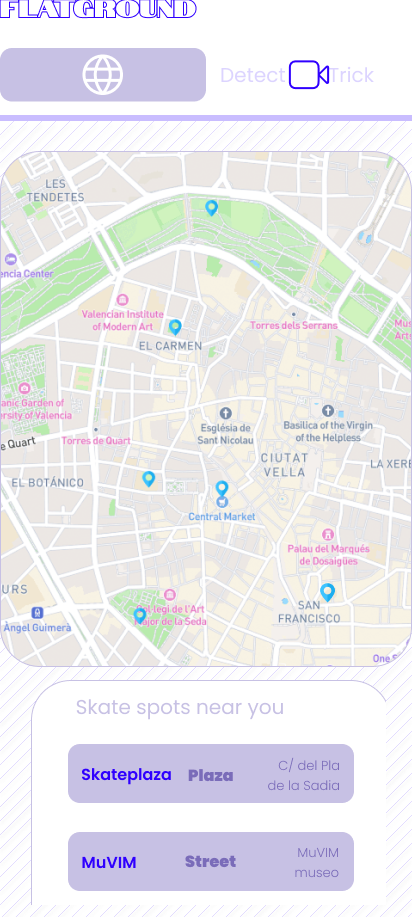
\includegraphics[width=0.4\linewidth]{Frame7.png}
                \caption{Makieta ekranu mapy aplikacji, Źródło: [Opracowanie własne].}
                \label{fig:app-map}
            \end{figure} 
            
            Zakładka podzielona jest na 2 części: interaktywną mapę, zajmującą większość ekranu oraz listę \enquote{spotów} deskorolkowych zlokalizowanych niedaleko od użytkownika. Na mapie widoczne są markery z lokalizacjami przeszkód i lokalizacja użykownika. Z kolei lista, pozwala na podgląd informacji na temat obiektów sportowych - nazwę, typ oraz adres.

        \subsubsection{Ekran wykrywania trików (\textit{Detect Trick})}

            Ekran dedykowany wykrywaniu trików, widoczny na rysunku \ref{fig:app-detect}, implementuje minimalistyczny i wysokokontrastowy design.

            \begin{figure}[!h]
                \centering 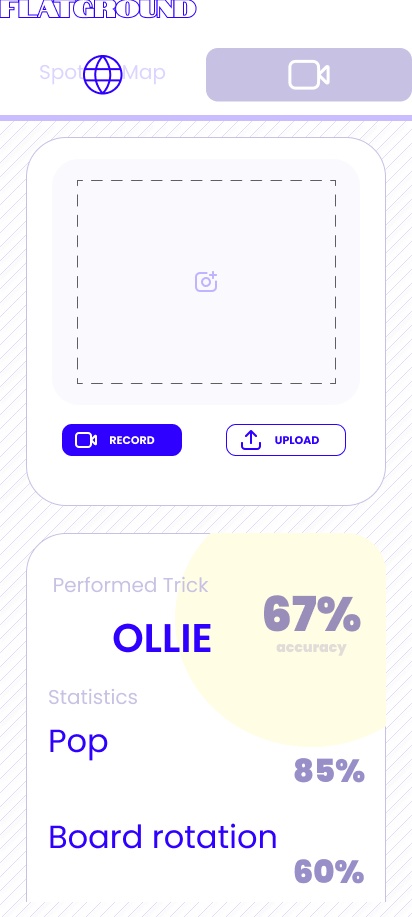
\includegraphics[width=0.4\linewidth]{KAMERA.png}
                \caption{Makieta ekranu detekcji triku aplikacji, Źródło: [Opracowanie własne].}
                \label{fig:app-detect}
            \end{figure}

            Ekran aplikacji podzielony został na 3 części:
            \begin{itemize}
                \item \textbf{Obsługa materiału wideo} - ta sekcja zawiera ramkę podglądu z dwoma wyraźnie widocznymi przyciskami: \textit{RECORD} (z ang. \enquote{nagraj}) i \textit{UPLOAD} (z ang. \enquote{importuj}). Taki układ dużych, czytelnych elementów minimalizuje ryzyko pomyłki i ułatwia obsługę smartfona jedną ręką;
                \item \textbf{Wyniki klasyfikacji} - sekcja pojawia się bezpośrednio pod modułem nagrywania. Kluczowa informacja, czyli rozpoznany trik (z ang. \textit{Performed Trick}), w tym przypadku \textit{Ollie}, jest zaprezentowana dużą czcionką. w centralnym miejscu ekranu, wraz z procentowym wskaźnikiem pewności klasyfikacji (z ang. \textit{Accuracy}). Na tym etapie projektowania przewidywano szczegółową analitykę w postaci statystyk technicznych: \textit{Pop} - siła wybicia, \textit{Board rotation} - rotacja deskorolki oraz \textit{Confidence} - pewność wykonywanego triku. Jednak ze względu na brak obiektywnych wzorców, na których można byłoby oprzeć takie statystyki, w późniejszych stadiach zrezygnowano z tych metryk;
                \item \textbf{Historia trików} - widoczna na rysunku \ref{fig:app-history} sekcja prezentuje użytkownikowi pięć ostatnich przeanalizowanych trików wraz z metryką \textit{Confidence}. Pozwala ona na szybkie przypomnienie ewolucji ćwiczonych w danej sesji treningowej oraz jej ustrukturyzowanie.
            \end{itemize}

            \begin{figure}[!h]
                \centering 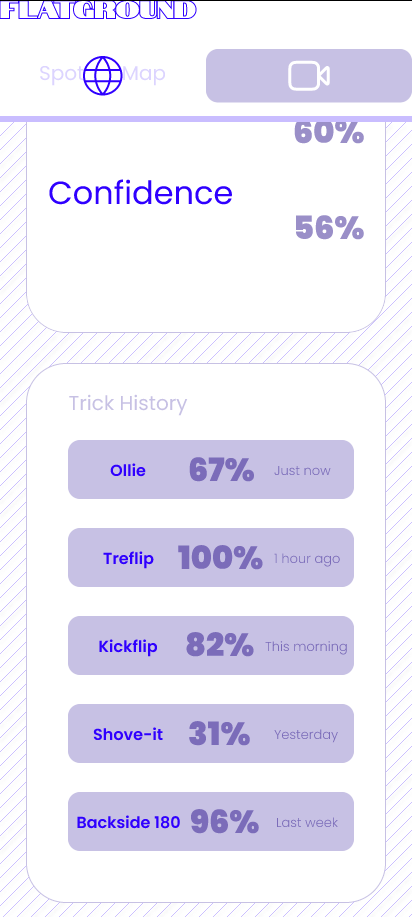
\includegraphics[width=0.4\linewidth]{historia.png}
                \caption{Makieta ekranu historii trików aplikacji, Źródło: [Opracowanie własne].}
                \label{fig:app-history}
            \end{figure}             

            Podział aplikacji na powyższe sekcje został podyktowany motywacją do stworzenia intuicyjnego i przejrzystego narzędzia treningowego. Zastosowana kolorystyka, oparta na odcieniach bieli i fioletu zapewnia wysoki kontrast, co było jednym z wymagań niefunkcjonalnych dotyczących czytelności interfejsu w warunkach oświetlenia zewnętrznego. Całość dąży do bycia \enquote{przezroczystym} narzędziem, które nie odciąga uwagi od treningu, a jedynie dostarcza niezbędnych danych w optymalnej formie.

    \subsection{Interakcja użytkownika z modułem rozpoznawania trików}

        W fazie projektowania w programie \textit{Figma} szczególną uwagę poświęcono interakcji użytkownika z narzędziem do analizy wizyjnej. Zaprojektowano sekwencyjny proces, który prowadzi użytkownika od momentu uruchomienia kamery, przez wybór pliku za pomocą komponentu \textit{image picker}, aż do prezentacji wyniku analizy.

        Interakcja z modułem SI została zaprojektowana w sposób asynchroniczny, co w praktyce inżynierskiej oznacza oddelegowanie zasobochłonnych obliczeń do zadań wykonywanych w tle, poza głównym wątkiem interfejsu użytkownika. Dzięki takiemu podejściu aplikacja zachowuje pełną responsywność - użytkownik nie doświadcza \enquote{zamrożenia} ekranu podczas analizy wizyjnej. W trakcie oczekiwania na wynik, w głównym oknie aplikacji wyświetlany jest podgląd zarejestrowanego materiału wideo, co pozwala na natychmiastową weryfikację nagrania przez sportowca.

        Finalny sposób prezentacji danych skupia się na dostarczeniu czytelnego sprzężenia zwrotnego w formie dashboardu analitycznego. Zamiast surowej reprezentacji szkieletowej, która mogłaby być nieczytelna dla użytkownika, system wyświetla nazwę rozpoznanego triku oraz szczegółowe metryki techniczne. Taka forma prezentacji ma na celu dostarczenie użytkownikowi obiektywnych danych o wykonanej ewolucji, co bezpośrednio realizuje założenie o stworzeniu bezinwazyjnego, mobilnego narzędzia wspomagającego trening. Wizualizacja ta została zoptymalizowana pod kątem użyteczności, zastępując skomplikowane wykresy prostymi wskaźnikami liczbowymi, co ułatwia szybką analizę błędów bezpośrednio po wykonaniu triku.

\newpage
\section{Opracowanie modułu sztucznej inteligencji}
    
    Niniejszy rozdział poświęcono szczegółowemu omówieniu procesu projektowania oraz implementacji modułu sztucznej inteligencji. Stanowi on główny silnik analityczny zaprojektowanej aplikacji mobilnej. Zgodnie z założeniami projektowymi opisanymi w rozdziale trzecim, klasyfikacja trików realizowana jest w oparciu o analizę wizyną działającą bezpośrednio na urządzeniu końcowym (w tym przypadku smarftonie użytkownika). Ze względu na złożoność tego zagadnienia, proces trworzenia systemu rozpoznawania ruchu podzielono na kilka kluczowych etapów, opisanych w kolejnych podrozdziałach. 
    
    \subsection{Zbiór danych treningowych}

        Do wytrenowania modelu klasyfikacyjnego wykorzystano ogólnodostępny zbiór danych wideo o nazwie \enquote{\textit{Skateboarding Trick Dataset (120fps)}}, udostępniony na platformie badawczej Kaggle \cite{kaggle_skateboarding_dataset}. Wybrany zbiór zawiera nagrania wideo przedstawiające osiem różnych klas ewolucji deskorolkowych: 
        \begin{itemize}
            \item Ollie,
            \item Kickflip,
            \item Heelflip,
            \item Frontside Shuvit,
            \item Shuvit,
            \item Backside 180,
            \item Frontside 180,
            \item Pressure Flip.
        \end{itemize}
        W zbiorze znajduje się po około pięćdziesiąt nagrań do każdej z klas.

        Początkowe plany projektowe zakładały rozbudowę bazy treningowe poprzez połączenie jej z zewnętrznymi materiałami, takimi jak repozytorium \textit{SkateboardML}, udostępnione w serwisie \textit{GitHub} przez użytkownika \textit{LightningDrop} \cite{lightningdrop2024}. Po dokładnej analizie danych źródłowych zdecydowano się jednak na odrzucenie tej koncepcji z uwagi na wysokie ryzyko błędów architektonicznych. Zewnętrzny zbiór zawierał po około 100 próbek wideo i ograniczał się tylko do dwóch klas (Ollie oraz Kickflip). Integracja tak ograniczonych danych ze zbalansowanym zbiorem z platformy \textit{Kaggle} mogłaby doprowadzić do drastycznego zaburzenia równowagi klas. Z punktu widzenia uczenia maszynowego skutkowałoby to wykształceniem przez sieć neuronową tzw. obciążenia (z ang. \textit{bias}) - model zacząłby sztucznie faworyzować te ewolucje, których próbek byłoby znacząco więcej niż innych (w tym przypadku Ollie i Kickflip). Przełożyłoby się to na znaczący wzrost liczby fałszywych detekcji podczas użytkowania aplikacji.

        Istotnym wyzwaniem inżynierskim była również rozbieżność w parametrach nagrań. Filmy z platformy \textit{Kaggle} były nagrywane z częstotliwością 120 klatek na sekundę (FPS - z ang. \textit{Frames per second}), podczas gdy aparaty docelowych urządzeń mobilnych pracują zazwyczaj w standardzie 30 FPS. Aby zapobiec wyuczeniu przez model nienaturalnie wolnej dynamiki ruchu, zastosowano w kodzie mechanizm odrzucania klatek, powodując tym samym konwersję wideo do 30 FPS.

        Należy zauważyć, że choć wielkość zastosowanego zbioru danych jest stosunkowo skromna jak na standardy komercyjnych systemów sztucznej inteligencji, jest to ilość w zupełności wystarczająca do opracowania funkcjonalnego prototypu (z ang. \textit{Proof of Concept}) i poprawnej walidacji koncepcji w ramach pracy inżynierskiej. Ewentualne powiększenie zbioru danych mogłoby w przyszłości zostać zrealizowane poprzez proces tzw. \textit{crowdsourcingu}, wykorzustując nagrania nadsyłane anonimowo przez aktywnych użytkowników aplikacji.

    \subsection{Ekstrakcja cech i estymacja pozy}

        Ze względu na wysoką złożoność obliczeniową surowych plików wideo, zdecydowano się na podejście oparte na detekcji cech przestrzennych szkieletu ludzkiego. Wykorzystano w tym celu model estymacji pozy \textit{Google MoveNet} pobrany z repozytorium \textit{TensorFlow Hub} \cite{openpose2025}. Model ten posiada dwa warianty:
        \begin{itemize}
            \item \textbf{Thunder}, w którym priorytetyzowana jest precyzja działania;
            \item \textbf{Lightning}, w przypadku którego kluczowa jest szybkość działania.
        \end{itemize}
        W przypadku niniejszej pracy inżynierskiej zdecydowano się na skorzystanie z wersji \textit{Thunder}, ponieważ w przypadku analizy tak dynamicznego i skomplikowanego ruchu, jakim jest jazda na deskorolce, wysoka precyzja jest kluczowa.

        Proces ekstrakcji pozy przebiegał w sposób ujednolicony dla każdej klatki. Najpierw obraz był skalowany i uzupełniany czarnymi pasami do wymiarów wejściowych wymaganych przez model, tj. 256x256 pikseli. Następnie \textit{MoveNet} przeprowadzał inferencję, lokalizując 17 kluczowych punktów szkieletu, takich jak stawy skokowe, kolanowe, ramiona czy biodra. Dla każdego punktu model zwraca trzy wartości: współrzędną X, współrzędną Y oraz współczynnik pewności wykrycia. W wyniku tej operacji każda klatka obrazu redukowana była do wektora jednowymiarowego składającego się z 51 cech numerycznych, co drastycznie obniżyło objętość danych przesyłanych do głównego klasyfikatora.

    \subsection{Preprocessing i normalizacja danych}
    
        Po ekstrakcji punkty kluczowe wymagały przekształcenia do postaci zrozumiałej dla modelu analizującego szeregi czasowe. Zebrane dane zostały uporządkowane chronologicznie, a etykiety tekstowe (nazwy trików) poddano kodowaniu numerycznemu za pomocą narzędzia \textit{LabelEncoder}.
        
        W celu uchwycenia dynamiki ruchu, zastosowana została technika przesuwnego okna (z ang. \textit{sliding window}). Rozmiar okna wejściowego ustawiono na 30 klatek, co przy znormalizowanej prędkości 30 FPS odpowiada dokładnie jednej sekundzie nagrania, co jest optymalnym czasem na wykonanie triku deskorolkowego. W celu powiększenia liczby unikalnych próbek, zastosowano przesunięcie okna o 2 klatki. Ostateczny zbiór danych składał się z trójwymiarowych tensorów o kształcie (30, 51) (30 klatek wideo, 51 cech w każdej klatce - iloczyn 17 punktów na ciele i 3 informacji dla każdego punktu), który następnie podzielono na zbiór treningowy i walidacyjny w klasycznej proporcji 80:20, gwarantując obiektywną ewaluację modelu. 

    \subsection{Architektura modelu klasyfikacyjnego}

        Na etapie doboru algorytmu decyzyjnego odrzucono ciężkie sieci rekurencyjne (np. \textit{LSTM}) na rzecz szybkiej, jednowymiarowej sieci neuronowej \textit{1D-CNN}. Sieci te zostały opisane szerzej w podrodziale 2.3, warto jednak zaznaczyć, iż wybrana architektura charakteryzuje się znacznie mniejszym zapotrzebowaniem na moc obliczeniową oraz zoptymalizowanym procesem wnioskowania, co bezpośrednio wpisuje się w założenia platformy docelowej, umożliwiając płynne działanie klasyfikatora lokalnie, wykorzystując wyłącznie moc obliczeniową procesora smartfona.

        Zaprojektowana sieć neuronowa składa się z następujących elementów operacyjnych:

        \begin{itemize}
            \item \textbf{Warstwa wejściowa}: przyjmująca sekwencje tensorów czasowo przestrzennych.
            \item \textbf{Pierwszy blok splotowy}: jednowymiarowa warstwa splotowa, wyodrębniająca lokalne wzorce ruchu przy użyciu 64 filtrów oraz nieliniowej funkcji aktywacji ReLU. Bezpośrednio za nią zastosowano warstwę odrzucania, dezaktywującą 30\% neuronów w celu zapobiegania zjawisku przeuczenia, oraz warstwę łączenia maksymalnego, odpowiedzialną za redukcję wymiarowości czasowej i wygładzenie rejestrowanego sygnału.
            \item \textbf{Drugi blok splotowy}: kolejna jednowymiarowa warstwa splotowa, poszerzona do 128 filtrów, zintegrowana z analogicznymi mechanizmami regularyzacji i zrzeszania przestrzennego.
            \item \textbf{Blok w pełni połączony}: warstwa spłaszczająca (z ang. \textit{Flatten}), dokonująca transformacji wyuczonych wielowymiarowych map cech do postaci wektora jednowymiarowego. Tak przetworzone dane przekazywane są do gęstej warstwy ukrytej, zbudowanej z 64 neuronów z funkcją aktywacji ReLU.
            \item \textbf{Warstwa wyjściowa}: warstwa gęsta wyposażona w 8 neuronów, których liczba odpowiada ilości rozpoznawanych klas ewolucji. Operuje ona na funkcji aktywacji \textit{Softmax}, która poddaje sygnały wyjściowe normalizacji, tworząc ostateczny rozkład prawdopodobieństwa przynależności analizowanej sekwencji do każdej z dyskretnych klas.
        \end{itemize}

    \subsection{Trenowanie modelu i konwersja TensorFlow Lite}

        Proces optymalizacji wag w zaprojektowanej sieci splotowej zrealizowano przy użyciu adaptacyjnego algorytmu optymalizacji \textit{Adam} (z ang. \textit{Adaptive Movement Estimation}). Algorytm ten dynamicznie dostosowuje czynniki uczenia dla poszczególnych wag na podstawie estymacji pierwszego i drugiego momentu gradientu, co pozwala na szybszą i bardziej stabilną zbieżność modelu. Celem optymalizacji była minimalizacja funkcji straty opartej na rzadkiej entropii krzyżowej (z ang. \textit{Sparse Categorical Crossentropy}). Proces uczenia zaplanowano na maksymalnie 50 epok, w trakcie których dane treningowe przetwarzano w mniejszych pakietach liczących po 32 próbki.

        W celu maksymalizacji zdolności modelu do generalizacji (poprawnego rozpoznawania nowych, nieznanych wcześniej nagrań) oraz zapobiegania zjawisku przeuczenia, zastosowano technikę regularyzacji zwaną wczesnym zatrzymywaniem. Polega ona na ciągłym monitorowaniu wartości funkcji straty na niezależnym zbiorze walidacyjnym po każdej epoce. Algorytm został zaprogramowany tak, aby automatycznie przerwać proces uczenia, jeżeli błąd walidacyjny nie uległ zmniejszeniu przez 10 kolejnych iteracji. Po takim zatrzymaniu, przywracane i zapisywane były te wagi sieci, dla których odnotowano najniższą wartość błędu, gwarantując wybór najbardziej optymalnego stanu modelu.

        Finalnym etapem prac nad silnikiem analitycznym była konwersja skomplikowanej sieci do lekkiego formatu binarnego, zoptymalizowanego pod kątem urządzeń o ograniczonych zasobach sprzętowych. W trakcie konwersji zastosowano rygorystyczne reguły kompilacji. Wymuszono mapowanie warstw sieci neuronowej wyłącznie na zbiór podstawowych operacji matematycznych, które są natywnie i sprzętowo wspierane przez procesory smartfonów. Tym samym zrezygnowano z implementacji złożonych, zewnętrznych instrukcji obliczeniowych macierzystej biblioteki programistycznej. Takie ograniczenie przestrzeni operacyjnej pozwoliło na znaczną redukcję objętości pliku wynikowego w formacie \textit{.tflite} oraz zagwarantowało wydajne, bezproblemowe wnioskowenia modelu na mobilnych architekturach procesorów.

%odnieść się do tego czy jest wystarczająca ilość danych treningowych
\newpage    
    \section{Budowa aplikacji mobilnej i warstwy serwerowej}

        Niniejszy rozdział poświęcono szczegółowemu opisowi architektury oras implementacji warstwy użytkownika systemu w postaci aplikacji mobilnej. Aplikacja ma na celu integrację funkcji mapowania skateparków z modułem analizy wizyjnej, realizującym wnioskowanie w czasie rzeczywistym na urządzeniu końcowym. W dalszej części rozdziału przedstawiono organizację kodu źródłowego, integrację interaktywnego modułu mapy,  sposób działania modułu analizującego i klasyfikującego nagrania trików deskorolkowych oraz architekturę integracji uczenia maszynowego.

    \subsection{Struktura projektu w środowisku Flutter}
        Aplikacja mobilna została zrealizowana z wykorzystaniem wielofplatformowego framework'a \textit{Flutter} oraz języka programowania \textit{Dart}. Wybór tej tej technologii ukierunkowany był przede wszystkim uniwersalnością (\textit{Flutter} działa zarówno na telefonach z systemem \textit{Android}, jak i \textit{iOS}). Ponadto posiada on możliwość kompilacji kodu źródłowego bezpośrednio do natywnych instrukcji procesorów o architekturze ARM, co zapewnia wysoką wydajność renderowania interfejsu użytkownika.

        Architekturę oprogramowania została zaprojektowana w oparciu o wzorzec podziału odpowiedzialności (z ang. \textit{Separation of concerns}), wyodrębniający trzy główne warstwy:
        \begin{enumerate}
            \item \textbf{Warstwę prezentacji} (\textit{UI}) odpowiedzialną za renderowanie komponentów interfejsu, zarządzanie stanem widoków oraz obsługę zdarzeń dotykowych użytkownika.
            \item \textbf{Warstwę logiki biznesowej i dziedzinowej} zawierającą struktury danych oraz algorytmy przetwarzania danych wejściowych.
            \item \textbf{Warstwę usług} realizującą komunikację sieciową z interfejsem \textit{API} (z ang. \textit{Application Programming Interface} - Interfejs programowania aplikacji) oraz niskopoziomowe operacje na urządzeniu końcowym (kamera, akceleratory uczenia maszynowego).
        \end{enumerate}

        W głównej funkcji programu (\texttt{main ()}) zaimplementowano wstępną konfigurację aplikacji. Za pomocą klasy \textit{SystemChrome} włączono trub pełoekranowy, ukrywając systemowe paski nawigacyjne. Pozwoliło to maksymalnie wykorzystać przestrzeń ekranu na potrzeby podglądu kamery oraz interaktywnej mapy. Spójność wizualną interfejsu zapowniono poprzez zdefiniowanie motywu głównego opartego na kroju pisma \textit{Poppins}.

    \subsection{Integracja modułu mapy}

        Moduł mapy odpowiada za wizualizację, rejestrację oraz edycję punktów reprezentujących skateparki, obiekty sportowe i \enquote{spoty} deskorolkowe. Warstwa komunikacji sieciowej została wyizolowana w ramach klasy \texttt{SkateSpotApi} operującej na protokole \texttt{HTTP} z wykorzystaniem architektury \texttt{RESTful}.    

        W celu ułatwienia testowania i wdrażania aplikacji, zaimplementowano funkcję dymanicznego wyboru adresu bazowego serwera (\texttt{\_resolveBaseUrl}). Metod ta sprawdza zmienne środowiskowe przekazane podczas kompilacji i automatycznie dobiera odpowiedni adres URL:
        \begin{itemize}
            \item dla środowiska lokalnego (deweloperskiego) kieruje zapytania pod adres IP emulatora Androida - \texttt{http://10.0.2.2:8000},
            \item dla środowiska produkcyjnego wykorzystuje adres serwera w chmurze (\textit{Render}),
        \end{itemize}
            Widoczna na poniższym załączniku metoda \texttt{\_resolveBaseUrl} odpowiada za dynamiczny dobór adresu bazowego \texttt{API}.

\begin{lstlisting}[
        language=Dart,
        caption={Metoda \texttt{\_resolveBaseUrl}.},
        label={lst:resolve_base_url}
    ]
static String _resolveBaseUrl({String? override}) {
if (override != null && override.isNotEmpty) {
    return override.replaceAll(RegExp(r'/$'), '');
}
const explicit = String.fromEnvironment('BACKEND_BASE_URL', defaultValue: '');
if (explicit.isNotEmpty) {
    return explicit.replaceAll(RegExp(r'/$'), '');
}
const appEnv = String.fromEnvironment('APP_ENV', defaultValue: 'dev');
if (appEnv == 'prod') {
    const prodUrl = String.fromEnvironment(
    'PROD_BACKEND_BASE_URL',
    defaultValue: 'https://flatground.onrender.com',
    );
    return prodUrl.replaceAll(RegExp(r'/$'), '');
}
return 'http://10.0.2.2:8000';
}
\end{lstlisting}

        Dane przesłane z serwera w formacie JSON są przekształcane na obiekty reprezentujące skateparki za pomocą klasy \texttt{SkateSpot}. \texttt{API} obsługuje pełen zestaw operacji \texttt{CRUD} (z ang. \textit{Create, Read, Update, Delete}), umożliwiając m. in. pobieranie listy obiektów wraz ze współrzędnymi geograficznymi, dodawanie szczegółowych opisów, określanie poziomu trudności oraz dołączanie zdjęć. Aby zapobiec awarii aplikacji w przypadku braku połączenia z internetem, zapytania sieciowe zabezpieczono obsługą błędów opartą na klasie \texttt{HttpException}.

    \subsection{Obsługa kamery i zarządzanie plikami wideo}
    
        Automatyczne rozpoznawanie trików wymaga pobrania i wstepnej obróbki nagrania z kamery smartfona. Z powodu dużej różnorodności modeli telefonów, powodującej dużą rozbieżność rozdzielczości i proporcji obrazu, materiał wideo przed przekazaniem do modli uczenia maszynowego musi zostać ustandaryzowany.

        Na proces przygotowania danych wideo składają sie dwa główne etapy:
        \begin{itemize}
            \item \textbf{Normalizacja przstrzenna klatek}: Każda klatka filmu ulega przeskalowaniu z zachowaniem oryginalnych proporcji obrazu, a następnie umieszczana w kwadratowej macierzy o wymiarach $256 x 256$ pikseli. Ewentualny wolny obszar powstały na skutek tej konwersji, uzupełniany jest czarnymi pasami, co zapobiega rozciąganiu czy spłaszczaniu sylwetki skatera. Takie zniekształcenie nagrania mogłoby zaburzyć dokładność detekcji punktów kluczowych przez model \textit{MoveNet}.
            \item \textbf{Normalizacja czasowa sekwencji}: Długości nagrań wgrywanych przez użytkowników różnią się od siebie, a główny klasyfikator wymaga wejścia o stałym wymiarze 30 klatek. Aby to osiągnąć, zaimplementowano funkcję \texttt{\_resampleKeypointSequence}, która przekształca sekwencję punktów kluczowych o dowolnej długości do wymaganego rozmiaru 30 klatek za pomocą liniowej interpolacji współrzędnych.
        \end{itemize}

        Na poniższym załączniku widoczny jest algorytm liniowej interpolacji i resamplingu sekwencji punktów kluczowych \texttt{\_resampleKeypointSequence}.

        \begin{lstlisting}[
                language=Dart,
                caption={Algorytm \texttt{\_resampleKeypointSequence}},
                label={lst:resolve_base_url}
            ]
List<List<double>> _resampleKeypointSequence(List<List<double>> source,
int targetLength) {
if (source.isEmpty) {
    return List.generate(targetLength, (_) => List.filled(51, 0.0));
}
if (source.length == targetLength) return source;
if (source.length == 1) {
    return List.generate(targetLength, (_) => List<double>.from(source.first));
}
final List<List<double>> out = [];
final double step = (source.length - 1) / (targetLength - 1);
for (int i = 0; i < targetLength; i++) {
    final pos = i * step;
    final left = pos.floor();
    final right = pos.ceil().clamp(0, source.length - 1);
    if (left == right) {
    out.add(List<double>.from(source[left]));
    continue;
    }
    final t = pos - left;
    final leftFrame = source[left];
    final rightFrame = source[right];
    final blended = List<double>.generate(
    51,
    (j) => leftFrame[j] * (1.0 - t) + rightFrame[j] * t,
    );
    out.add(blended);
}
return out;
}\end{lstlisting}

        Pliki wideo nie są przechowywane w pamięci urządzenia ze względu na brak użytecznego uzasadnienia takiego rozwiązania oraz potencjalne zużywanie zasobów pamięci urządzenia w przypadku nagromadzenia znacznej ilości nagrań. Zamiast tego, użytkownik ma dostęp do historii pięciu ostatnich trików, wraz ze stopniem pewności modelu co do klasyfikacji triku, wyrażonej w warości procentowej.

    \subsection{Integracja modułu TensorFlow Lite z aplikacją}
    \subsection{Architektura i impelemtacja warstwy serwerowej}
    \subsection{Baza danych oraz przechowywanie zasobów multimedialnych}

\newpage
\section{Testy oraz analiza wyników}
    W poniższym rozdziale przedstawiono przebieg testów aplikacji mobilnej, warstwy serwerowej oraz modułu klasyfikacji trików. Celem testów było sprawdzenie, jak zaprojektowany system zachowuje się w praktyce, zestawienie rzeczywistej skuteczności sieci neuronowej z wynikami z fazy treningowej oraz zidentyfikowanie obszarów wymagających poprawek.

    \subsection{Środowisko testowe}

        Testy aplikacji mobilnej przeprowadzono na dwóch fizycznych urządzeniach z systemem \textit{Android}: smartfonie \textit{Mode1 Retro II} oraz \textit{Samsung Galaxy S21}, a także na wirtualnym emulatorze w środowisku \textit{Android Studio}. Model uczenia maszynowego był uruchamiany przy użyciu biblioteki \textit{TensorFlow Lite Runtime}.

        Warstwę serwerową przetestowano za pomocą automatycznych testów w języku \textit{Python}, wykorzystując do tego bibliotekę \texttt{pytest}. Zastosowano do tego izolowane środowisko z bazą danych \textit{SQLite} w pamięci, co pozwalało symulować docelową bazę \textit{PostgreSQL} bez modyfikacji rzeczywistych danych.

    \subsection{Ewaluacja skuteczności modelu sztucznej inteligencji}

        W fazie trenowania i walidacji model osiągnął skuteczność na poziomie 96\%, co zostało szerzej omówione w rozdziale 5. Głównym celem poniższych testów było sprawdzenie, jak ten wynik przełoży się na działanie aplikacji na docelowym urządzeniu mobilnym.

        \subsubsection{Scenariusze testowe i zbiór ewaluacyny}

            Do ewaluacji przygotowano własny zbiór 50 nagrań wideo. Filmy zostały zarejestrowane testowymi smartfonami w rozdzielczości 1080p przy 30 klatkach na sekundę. Ponadto wykorzystane zostały archiwalne nagrania, zgromadzone przez autora pracy. W celu rzetelnej reprezentacji rzeczywistego wykorzystywania aplikacji, nagrania testowe charakteryzowały się zróżnicowanymi warunkami oświetleniowymi, odległością kamerującego od sportowca oraz kątem nagrywania. Za sukces uznawano sytuację, w której algorytm poprawnie rozpoznał wykonany trik z pewnością wynoszącą co najmniej 75\%. Wyniki poniżej tego progu aplikacja traktuje jako nierozpoznane, więc w trakcie testów przyjęto takie samo założenie.
            
        \subsubsection{Wyniki klasyfikacji i ich analiza}

            Na 50 przeprowadzonych prób, model poprawnie sklasyfikował 38 z nich, co odpowiada skuteczności na poziomie 76\%. Oznacza to spadek skuteczności o 20 punktów procentowych względem wyników uzyskanych w fazie treningowej. Wyniki dla poszczególnych trików oraz zestawienie popełnionych błędów przedstawiono w tabeli \ref{tab:field_tests}.

            \begin{table}[!ht] \centering
                \caption{Wyniki testów polowych klasyfikatora na zbiorze 50 nagrań ze smartfonów.}
                \label{tab:field_tests} 
                \begin{tabularx}{\textwidth}{ | l | c | c | X | c | } \hline
                    \textbf{Klasa ewolucji} & \textbf{Liczba prób} & \textbf{Poprawne} & \textbf{Błędne klasyfikacje (Szczegóły)} & \textbf{Skuteczność} \\ \hline
                    Ollie & 10 & 9 & 1x sklasyfikowano jako Kickflip & 90\% \\ \hline
                    Kickflip & 8 & 5 & 2x jako Ollie, 1x jako Heelflip & 62,5\% \\ \hline
                    Heelflip & 7 & 5 & 2x jako Ollie & 71\% \\ \hline
                    Shuvit & 6 & 4 & 1x jako Frontshuvit, 1x Nierozpoznany & 66\% \\ \hline
                    Frontshuvit & 5 & 4 & 1x jako Shuvit & 80\% \\ \hline
                    Frontside 180 & 5 & 5 & Brak błędów & 100\% \\ \hline
                    Backside 180 & 5 & 4 & 1x Nierozpoznany & 80\% \\ \hline
                    Pressure Flip & 4 & 2 & 1x jako Shuvit, 1x Nierozpoznany & 50\% \\ \hline
                    \textbf{SUMA} & \textbf{50} & \textbf{38} & \textbf{12 błędów (w tym 3 nierozpoznane)} & \textbf{76\%} \\ \hline
                \end{tabularx}
            \end{table}

            Z zebranych danych wynika, że najlepiej rozpoznawanym trikiem jest \textit{Frontside 180}, przy którym nie zarejstrowano żadnej błędnej klasyfikacji. Słabsze wyniki uzyskano dla trików polegających na obrocie deski, czyli: \textit{Kickflip} (62,5\%), \textit{Heelflip}(71\%) oraz \textit{Pressure Flip}(50\%). Model najczęściej mylił je z \textit{Ollie}, co może być spowodowane podobnym ruchem tułowia w trakcie wykonywania tych trików. Dodatkowo, ograniczenia aparatów w smartfonach mogą powodować problemy z rejestrowaniem szybkiego ruchu stopy, który jest kluczowy w odróżnianiu tych sztuczek od siebie nawzajem. W przypadku błędnej klasyfikacji trików z obrotem deski, algorytm \textit{MoveNet} gubił pozycję stóp, co powodowało rejestrację jedynie podskoku sylwetki, pomijając charakterystyczne kopnięcie, które wprawia deskorolkę w obrót.

            Warto również odnotować, że trzy próby zostały przez aplikację odrzucone z powodu pewności niższej niż 75\%. Z punktu widzenia użytkowego jest to zjawisko pożądane, ponieważ pomaga uniknąć wprowadzania użytkownika aplikacji w błąd.

            Rzeczywistą skuteczność na poziomie 76\% można uznać za zadowalającą dla pierwszej wersji aplikacji. Ewentualna poprawa tych wyników wymagałaby zgromadzenia znacznie większej ilości zróżnicowanych danych treningowych, co mogłoby być osiągnięte za pomocą \textit{crowdsourcingu}, czyli gromadzenia nagrań od użytkowników aplikacji i uczenie modelu za ich pomocą.
            
    \subsection{Testy funkcjonalne aplikacji mobilnej}

            Po sprawdzeniu modelu sztucznej inteligencji, przetestowano działanie samej aplikacji mobilnej oraz integracji z backendem.

            \subsubsection{Scenariusze i przypadki testowe}

                Do weryfikacji interfejsu użytkownika i logiki biznesowej przygotowano cztery manualne przypadki testowe, które miały sprawdzić najważniejsze funkcje systemu:
                \begin{itemize}
                    \item \textbf{Scenariusz 1}: Dodanie nowego \enquote{spotu} z opisem, zdjęciem, współrzędnymi, nazwą i poziomem trudności, a nastepnie sprawdzenie czy pojawi się on poprawnie na mapie na drugim urządzeniu/
                    \item \textbf{Scenariusz 2}:
                \end{itemize}
\newpage
\section{Podsumowanie}

    Głównym celem niniejszej pracy inżynierskiej było zaprojektowanie i wdrożenie aplikacji mobilnej wspierającej sportowców uprawiających jazdę na deskorolce. Proces ten obejmował stworzenie interaktywnej mapy \enquote{spotów} deskorolkowych oraz modułu klasyfikacji trików opartego na analizie wizyjnej. Wdrożenie tego systemu dowiodło, że współczesne urządzenia mobilne, nawet te o ograniczonych zasobach obliczeniowych, dysponują wystarczającą mocą obliczeniową do uruchamiania modeli uczenia maszynowego lokalnie, bez konieczności ciągłego dostępu do internetu. Na podstawie wniosków wyciągnietych z testowania, wdrożono modyfikacje, których skutkiem było znaczące zredukowanie czasu analizy trików oraz płynniejsze doświadczenie użytkownika. Udało się zidentyfikować błędy, które niewykryte znacząco utrudniałyby korzystanie ze wszystkich funkcjonalności stworzonej aplikacji. Pozostałe testy potwierdziły poprawność działania innych części systemu.

    Pomimo pozytywnej weryfikacji głównych założeń systemu, przeprowadzone testy praktyczne ukazały techniczne i sprzętowe ograniczenia stworzonego rozwiązania. Odnotowano zauważalny spadek skuteczności z 96\% uzyskanych podczas trenowania klasyfikatora do praktycznej dokładności wynoszącej 80\%. Spadek ten mógł być spowodowany zarówno parametrami aparatów wbudowanych w smartfony, złą techniką i warunkami w trakcie tworzenia nagrań oraz zbyt małym zbiorem danych treningowych. Nagrania w złym oświetleniu często charakteryzują się rozmyciem w ruchu, co negatywnie wpływa na działanie modelu \textit{MoveNet}. Detekcja pozy, a szczególnie prawidłowa detekcja i precyzyjne śledzenie ruchu stóp jest kluczowe w wykrywaniu trików opartych na szybkiej rotacji deskorolki, takich jak \textit{Kickflip} oraz \textit{Heelflip}. Ograniczeniem projektowym był również wspomniany już relatywnie niewielki zbiór danych treningowych, liczący około 400 nagrań. Baza wideo z platformy \textit{Kaggle} zawężała zdolność sieci neuronowej do radzenia sobie z okluzją, zmiennymi kątami kamery oraz słabymi warunkami oświetleniowymi, mimo tego, iż była to największa taka baza znaleziona przez autora pracy.
    
     % wystarczy podmienić swoje pliki main.tex i eiti-thesis.cls
                            % na nowe wersje, a cały tekst pracy pozostaje nienaruszony.

%--------------------------------------------
% Literatura
%--------------------------------------------
\cleardoublepage % Zaczynamy od nieparzystej strony
\printbibliography

%--------------------------------------------
% Spisy (opcjonalne)
%--------------------------------------------
\newpage
\pagestyle{plain}

% Wykaz symboli i skrótów.
% Pamiętaj, żeby posortować symbole alfabetycznie
% we własnym zakresie. Ponieważ mało kto używa takiego wykazu,
% uznałem, że robienie automatycznie sortowanej listy
% na poziomie LaTeXa to za duży overkill.
% Makro \acronymlist generuje właściwy tytuł sekcji,
% w zależności od języka.
% Makro \acronym dodaje skrót/symbol do listy,
% zapewniając podstawowe formatowanie.
% //AB
\vspace{0.8cm}


\listoffigurestoc     % Spis rysunków.
\newpage         % vertical space
\listoftablestoc      % Spis tabel.
\newpage          % vertical space
%\listofappendicestoc  % Spis załączników

% Załączniki
% \newpage
% \appendix{Nazwa załącznika 1}
% \lipsum[1-8]

% \newpage
% \appendix{Nazwa załącznika 2}
% \lipsum[1-4]

% Używając powyższych spisów jako szablonu,
% możesz tu dodać swój własny wykaz bądź listę,
% np. spis algorytmów.

\end{document} % Dobranoc.
